% =============================================================================
% sup_appendix.tex — the supplemental (online) appendix, shared body.
%   Appendix C: additional descriptive evidence.
%   Appendix D: robustness, measurement, and inference.
%   Appendix E: the policy record (design failures, not program evaluations).
% Compiled two ways: \input by supplement.tex (standalone online supplement), and
% by Born_on_Schedule.tex (the working paper). Numbering (C, D, E) is set by
% \numberwithin in the host preamble. Table captions and notes live in
% analysis/code/00_table_text.R, not here.
% =============================================================================

% =============================================================================
\section{Additional descriptive evidence}\label{app:descriptive}
% =============================================================================

The descriptive exhibits document the populations and patterns underlying the
paper's analysis. They do not establish the causal effect of scheduling.
Table~\ref{tab:descriptives} describes the municipality-year sample used to
estimate the fee relationship, and Figure~\ref{fig:map_private} shows the
geographic distribution of private-insurance cesarean rates.
Tables~\ref{tab:business_hours} and~\ref{tab:mechanism_checks} and
Figures~\ref{fig:robson_dow} and~\ref{fig:daily_counts} characterize the weekly
concentration of surgical deliveries. Figure~\ref{fig:gestation} compares
gestational-age distributions. Table~\ref{tab:estab_practice_style} measures
between-establishment variation after standardizing the Robson-group
distribution, and Table~\ref{tab:cost} reports gross amounts billed for delivery
hospitalizations.

\begin{table}[H]\centering
\caption{\textbf{Municipality-year summary statistics}}\label{tab:descriptives}
\small
\small\setlength{\tabcolsep}{4pt}\resizebox{\ifdim\width>\linewidth \linewidth\else\width\fi}{!}{%
\begin{tabular}{lrrrrrr}
\toprule
Variable & Mean & Std.\ dev. & 10th pct. & Median & 90th pct. & $N$ \\
\midrule
Cesarean rate, private (TISS) & 0.84 & 0.09 & 0.73 & 0.85 & 0.94 & 5,198 \\
Cesarean rate, for-profit (SINASC) & 0.82 & 0.11 & 0.68 & 0.83 & 0.95 & 2,823 \\
Log economic fee gap (cesarean minus vaginal) & -0.04 & 0.38 & -0.42 & -0.08 & 0.44 & 5,198 \\
Obstetricians per 1,000 births & 24.02 & 70.92 & 11.09 & 20.97 & 35.09 & 5,189 \\
GDP per capita (R\$ thousands) & 65.97 & 30.37 & 33.71 & 62.13 & 91.88 & 4,715 \\
Private health-plan coverage (\%) & 38.78 & 12.25 & 21.23 & 40.02 & 53.25 & 5,198 \\
Adequate prenatal care (\%) & 70.31 & 10.66 & 55.10 & 73.12 & 81.39 & 5,198 \\
\bottomrule
\end{tabular}
}
\begin{minipage}{\linewidth}\footnotesize
\textit{Notes:} The sample comprises municipality-years from 2015 to 2024 with at least 20 private-insurance deliveries and a defined relative physician fee, the sample of the fee regressions. Means and percentiles are weighted by the number of TISS deliveries, as in the fee regressions. TISS is the private-insurance claims database; the establishment-sector measure comes from SINASC linked to CNES. The unweighted mean log economic fee gap is +0.21, whereas the delivery-weighted mean is $-0.04$: smaller municipalities more often have positive gaps, but 57 percent of private-insurance deliveries occur where cesareans have lower expected physician fees than vaginal deliveries.
\end{minipage}
\end{table}


\begin{figure}[H]\centering
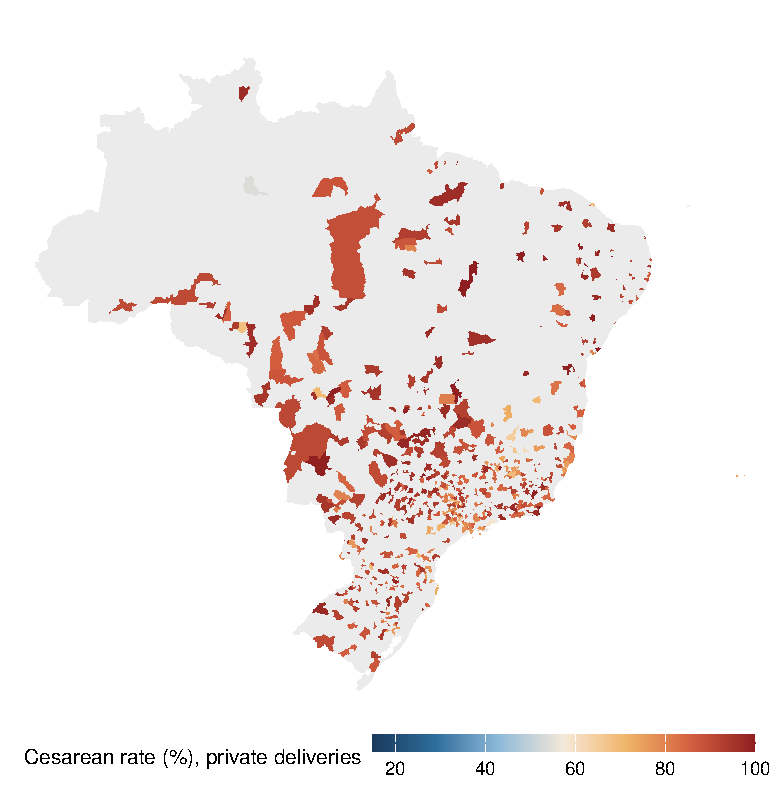
\includegraphics[width=0.8\textwidth]{../analysis/output/maps/map02_csection_private.pdf}
\caption{\textbf{Private-insurance cesarean rate by municipality}}\label{fig:map_private}
\fignotes{TISS deliveries, 2020--2024, attributed to the municipality of the
provider. Rates are mapped for municipalities with at least 100 deliveries during
the period; the remaining municipalities are shown in gray. The unit is the
private-insurance delivery, not a SINASC birth classified by establishment
ownership.}
\end{figure}

\begin{table}[H]\centering
\caption{\textbf{Share of births during weekday business hours}}
\label{tab:business_hours}
\small
\begin{tabular}{lcc}
\toprule
Sector & Cesarean & Vaginal \\
\midrule
For-profit & 50.1\% & 33.2\% \\
Public & 50.9\% & 32.0\% \\
\midrule
Uniform-timing benchmark & \multicolumn{2}{c}{29.8\%} \\
\bottomrule
\end{tabular}
\begin{minipage}{\linewidth}\footnotesize
\textit{Notes:} SINASC live births, 2010--2024, with a recorded delivery time. Business hours are Monday--Friday, 8:00--17:59. If births were distributed uniformly across all hours of the week, 29.8 percent would occur in this interval. The cesarean concentration is almost identical across ownership sectors, which is inconsistent with reading all weekday timing as the personal convenience of for-profit physicians alone.
\end{minipage}
\end{table}


\begin{figure}[H]\centering
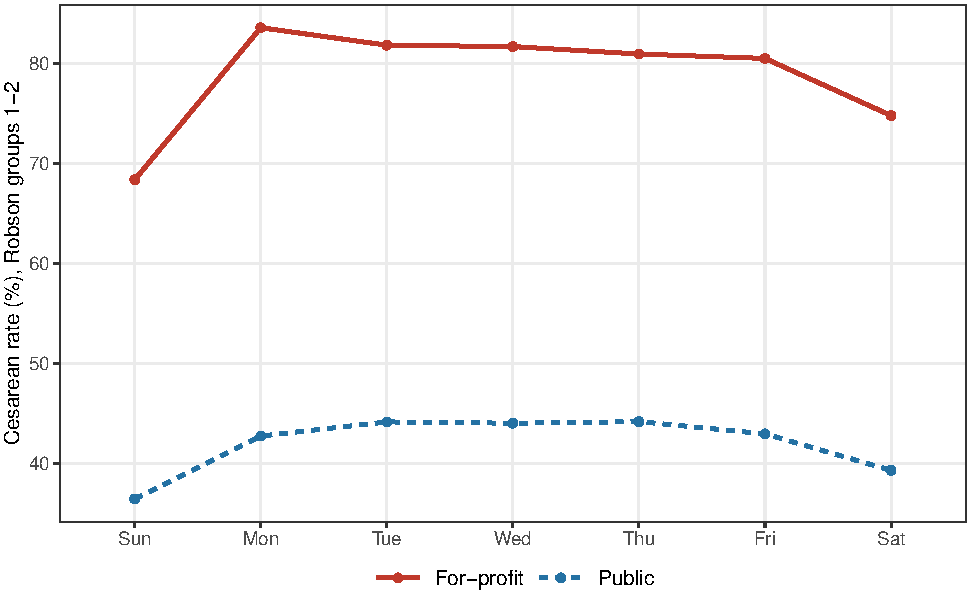
\includegraphics[width=\textwidth]{../analysis/output/graphs/fig03_robson_dow.pdf}
\caption{\textbf{Cesarean rates over the week, Robson groups 1--2}}\label{fig:robson_dow}
\fignotes{SINASC, 2014--2024, the years for which the Robson classification is
populated. The figure includes groups 1--2 (nulliparous women with term,
singleton, cephalic pregnancies) and describes the day-of-week pattern separately
for public and for-profit establishments; differences across days are not
adjusted for patient sorting within the groups.}
\end{figure}

\begin{figure}[H]\centering
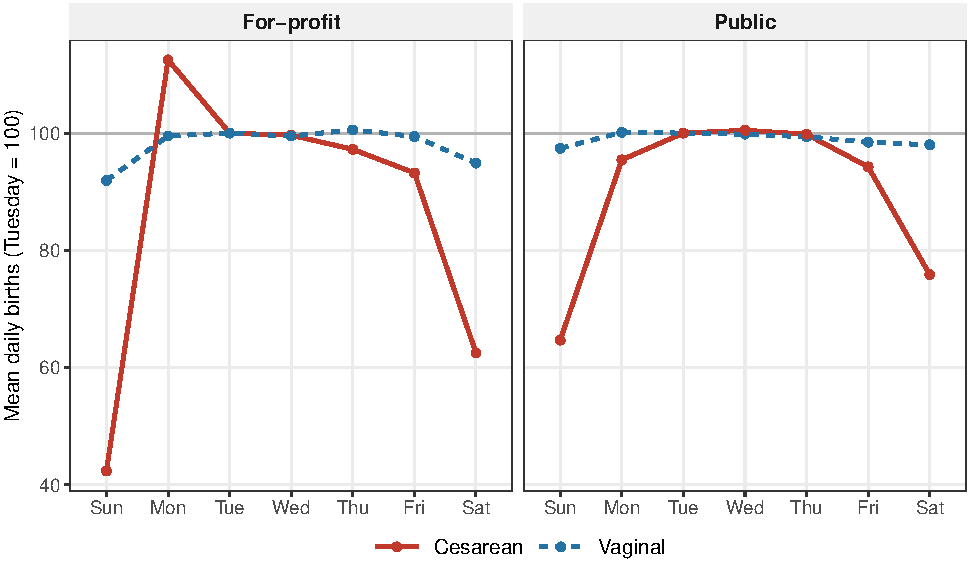
\includegraphics[width=\textwidth]{../analysis/output/graphs/fig08_daily_counts.pdf}
\caption{\textbf{Daily delivery counts by mode and sector}}\label{fig:daily_counts}
\fignotes{SINASC mean delivery counts, with each series indexed to Tuesday $=100$.
Cesarean counts fall substantially on weekends in both ownership sectors, whereas
vaginal counts vary much less. These counts complement the cesarean-share
regressions: a falling share alone would not establish that fewer cesareans take
place.}
\end{figure}


\begin{sidewaystable}\centering
   \caption{\label{tab:mechanism_checks} \textbf{Weekend gradients by cesarean timing and Robson group}}
   \centering
\small\setlength{\tabcolsep}{4pt}\resizebox{\ifdim\width>\linewidth \linewidth\else\width\fi}{!}{%
   \begin{tabular}{lcccccc}
      \toprule
 & (1)             & (2)            & (3)             & (4)             & (5)                & (6)\\  
\addlinespace[2pt]
 & Prelabor cesarean share & In-labor cesarean share & Prelabor cesarean share & In-labor cesarean share & \multicolumn{2}{c}{Cesarean share}\\
      \midrule
      Weekend      & -0.0893$^{***}$ & 0.0186$^{***}$ & -0.0432$^{***}$ & -0.0143$^{***}$ & -0.0703$^{***}$    & -0.0478$^{***}$\\   
                   & (0.0063)        & (0.0038)       & (0.0024)        & (0.0016)        & (0.0042)           & (0.0030)\\   
\addlinespace[2pt]
      Sector       & For-profit      & For-profit     & Public          & Public          & For-profit         & For-profit\\  
      Sample       & All births      & All births     & All births      & All births      & Robson groups 1--2 & Robson group 10 (preterm)\\  
      \midrule
      Municipality fixed effects & Yes             & Yes            & Yes             & Yes             & Yes                & Yes\\  
      Year fixed effects & Yes             & Yes            & Yes             & Yes             & Yes                & Yes\\  
      \midrule
      Observations & 1,201,826       & 1,201,826      & 3,099,291       & 3,099,291       & 627,120            & 261,262\\  
\bottomrule
   \end{tabular}
}
\begin{minipage}{\linewidth}\footnotesize
\textit{Notes:} SINASC municipality-date cells, weighted by births. Columns 1--4 cover 2012--2024 and divide the cesarean share into procedures recorded as performed before labor and procedures recorded during labor. Cesareans with missing or invalid timing codes remain in the denominator but enter neither timing-specific numerator. Columns 5--6 cover 2014--2024 and compare Robson groups 1--2 with group 10 (preterm births). A preterm delivery may itself be planned; group 10 is therefore a comparison group, not a placebo in which scheduling is impossible. Standard errors, two-way clustered by municipality and date, are reported in parentheses.
\newline
\footnotesize Significance levels: *** $p<0.01$, ** $p<0.05$, * $p<0.10$.
\end{minipage}
\end{sidewaystable}




\begin{figure}[H]\centering
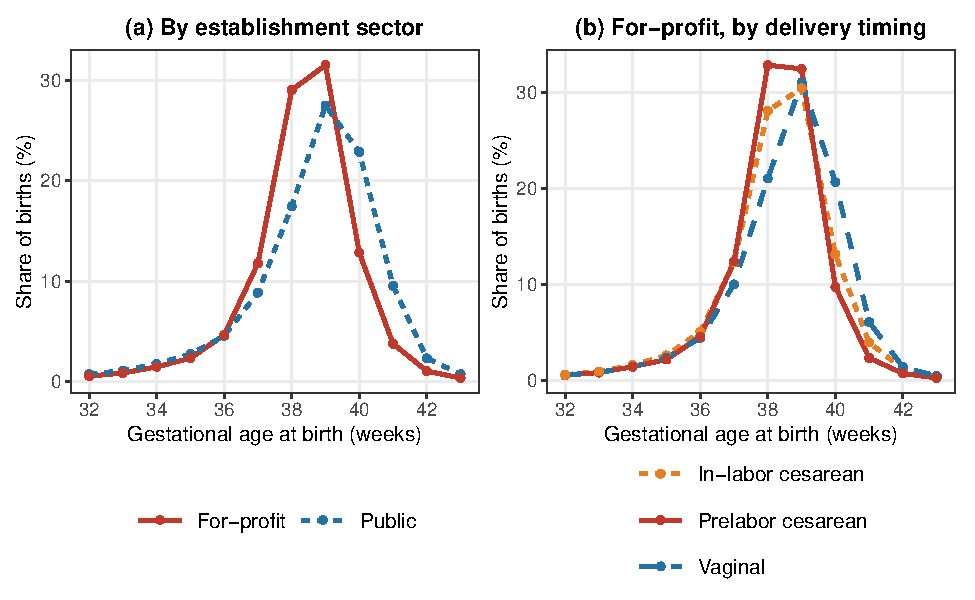
\includegraphics[width=\textwidth]{../analysis/output/graphs/fig_gestation_panels.pdf}
\caption{\textbf{Gestational age at birth}}\label{fig:gestation}
\fignotes{SINASC, 2010--2024, for panel (a); 2012--2024 for the timing breakdown
in panel (b). Both sectors' modal gestational age is 39 completed weeks. Relative
to public births, the for-profit distribution is shifted toward earlier gestation:
about 41 versus 26 percent of births occur at 37--38 weeks, and 17 versus 32
percent at 40--41 weeks. Within for-profit establishments, the early-term shares
are about 45 percent for prelabor cesareans, 40 percent for in-labor cesareans,
and 31 percent for vaginal deliveries. These are three distinct distributions, and
in-labor cesareans should not be grouped with vaginal deliveries. The figure
describes timing associations, not the causal effect of scheduling on gestational
age.}
\end{figure}

\begin{table}[H]\centering
\caption{\textbf{Between-establishment variation after Robson standardization}}
\label{tab:estab_practice_style}
\footnotesize\setlength{\tabcolsep}{4pt}\resizebox{\ifdim\width>\linewidth \linewidth\else\width\fi}{!}{%
\begin{tabular}{lrrrrrrrr}
\toprule
 & & & \multicolumn{3}{c}{Observed rate (\%)} & \multicolumn{3}{c}{Robson-standardized (\%)} \\
\cmidrule(lr){4-6}\cmidrule(lr){7-9}
 & Establishment- & & & & P90$-$ & & & P90$-$ \\
 & years & Births & Mean & SD & P10 & Mean & SD & P10 \\
\midrule
\multicolumn{9}{l}{\emph{Panel A. Dispersion across establishments, by sector}} \\
\addlinespace[2pt]
For-profit & 6,104 & 5,619,532 & 80.2 & 15.3 & 37.9 & 73.0 & 14.1 & 36.7 \\
Nonprofit & 9,440 & 9,990,289 & 60.7 & 18.0 & 47.8 & 58.7 & 14.4 & 36.4 \\
Public & 10,419 & 12,394,594 & 45.1 & 14.8 & 36.1 & 48.0 & 12.6 & 30.8 \\
\addlinespace[4pt]
\midrule
\multicolumn{9}{l}{\emph{Panel B. Dispersion of the standardized rate surviving each block}} \\
\addlinespace[2pt]
 & \multicolumn{3}{c}{All sectors} & & \multicolumn{3}{c}{For-profit only} & \\
\cmidrule(lr){2-4}\cmidrule(lr){6-8}
 & $R^2$ & Residual SD & \% of raw & & $R^2$ & Residual SD & \% of raw & \\
\midrule
None (raw dispersion) &  & 16.25 & 100 &  &  & 14.09 & 100 &  \\
Sector & 0.310 & 13.51 & 83 &  &  &  &  &  \\
$+$ Municipality $\times$ year & 0.759 & 7.97 & 49 &  & 0.731 & 7.31 & 52 &  \\
$+$ Maternal case-mix & 0.868 & 5.92 & 36 &  & 0.792 & 6.42 & 46 &  \\
$+$ Obstetric capacity & 0.870 & 5.85 & 36 &  & 0.803 & 6.26 & 44 &  \\
\bottomrule
\end{tabular}
}
\begin{minipage}{\linewidth}\footnotesize
\textit{Notes:} SINASC 2014--2024; establishment-years with at least 100 births, weighted by births. Each establishment's group-specific cesarean rates are reweighted to the national Robson-group distribution of the same year. Establishments are retained if the groups they serve cover at least 90 percent of the reference distribution; weights are renormalized over those groups. Panel A compares observed and standardized dispersion across establishments. Panel B uses the standardized rate as its outcome and reports the share of its variance explained and the residual weighted standard deviation after progressively controlling for establishment sector, municipality-by-year, maternal composition, and obstetric capacity. All rows of Panel B use the same complete-case sample of 23,056 establishment-years. Maternal controls comprise mean age and the shares under 20, aged 35 or above, with no more than seven years of schooling, and not recorded as white. Capacity includes CNES obstetric beds and delivery volume. The for-profit columns omit the sector indicator by construction. Regressing the unstandardized rate directly on Robson shares would absorb both clinical mix and correlated within-group practice, overstating what observed case-mix explains. Two for-profit establishments delivering in the same municipality and year differ by 11.9 percentage points on average in the standardized rate. The residual variation is not a causal measure of physician practice style: it also includes unmeasured case-mix, staffing, and establishment organization.
\end{minipage}
\end{table}


Standardization narrows the between-sector gap but leaves substantial dispersion
within ownership categories. Among for-profit establishments, the standard
deviation of the standardized rate is 14.1 percentage points. After
municipality-by-year effects, maternal controls, and measured capacity, 44 percent
of the original dispersion remains (Table~\ref{tab:estab_practice_style},
Panel B). Establishments operating in the same market can thus differ markedly in
cesarean intensity even after standardization, but the data do not identify which
part of that difference is attributable to individual clinicians.

\begin{table}[H]\centering
\caption{\textbf{Total amount billed per delivery hospitalization}}
\label{tab:cost}
\small
\small\setlength{\tabcolsep}{4pt}\resizebox{\ifdim\width>\linewidth \linewidth\else\width\fi}{!}{%
\begin{tabular}{lcc}
\toprule
 & Cesarean & Vaginal \\
\midrule
Mean billed amount (R\$) & 6,992 & 7,093 \\
Median billed amount (R\$) & 5,633 & 5,438 \\
Deliveries, 2015--2024 & 2,828,828 & 543,736 \\
\bottomrule
\end{tabular}
}
\begin{minipage}{\linewidth}\footnotesize
\textit{Notes:} TISS hospitalization claims, 2015--2024. Amounts sum the reported charges for procedures, materials, drugs, daily hospital rates, and other billing items under each delivery event; the upper and lower 0.5 percent of the distribution are trimmed. They are gross billed amounts, not negotiated insurer payments, costs of production, or hospital profits. Mean billed amounts are close across delivery modes, and the median is modestly higher for cesareans. These comparisons cannot establish the relative profitability of the procedures.
\end{minipage}
\end{table}


% =============================================================================
\section{Robustness, measurement, and inference}\label{app:robustness}
% =============================================================================

The results in the paper describe differences in the timing and mode of delivery.
The exercises below test whether those patterns survive alternative definitions
and samples, how much of the ownership differential arises within hospitals, and
what the data can and cannot say about competing explanations. They also document
fee measurement and statistical inference.

\subsection{Alternative samples, composition, and clinical subgroups}

The for-profit weekend dip is not specific to the preferred legal-entity
classification or to a Saturday--Sunday indicator. Reclassifying establishments as
for-profit if they were for-profit in any year produces a weekend estimate of
$-8.2$ percentage points; using Sunday alone gives $-10.4$ points, and combining
weekends and holidays gives $-7.7$ points (Table~\ref{tab:referee_robustness}).
These definitions measure different rest-day contrasts and should not be treated
as interchangeable estimates of the same exposure. Weekend births in for-profit
establishments also have higher low-Apgar and low-birthweight shares, consistent
with nonrandom sorting of deliveries across days rather than with changes in
health caused by delivery on those days.


\begin{sidewaystable}\centering
   \caption{\label{tab:referee_robustness} \textbf{Weekend gradients under alternative definitions and newborn composition}}
   \centering
\footnotesize\setlength{\tabcolsep}{3pt}\resizebox{\ifdim\width>\linewidth \linewidth\else\width\fi}{!}{%
   \begin{tabular}{lccccc}
      \toprule
 & (1)                                   & (2)                        & (3)                      & (4)                  & (5)\\  
\addlinespace[2pt]
 & \multicolumn{3}{c}{Cesarean rate} & \multicolumn{2}{c}{Newborn outcome}\\
      \cmidrule(lr){2-4}\cmidrule(lr){5-6}
                                    & Cesarean rate, for-profit in any year & Cesarean rate, Sunday only & Cesarean rate, rest days & Low Apgar (5-minute) & Low birthweight \\   
\addlinespace[2pt]
      \midrule
      Weekend                       & -0.0821$^{***}$                       &                            &                          & 0.0018$^{***}$       & 0.0133$^{***}$\\   
                                    & (0.0050)                              &                            &                          & (0.0002)             & (0.0012)\\   
\addlinespace[2pt]
      Sunday                        &                                       & -0.1038$^{***}$            &                          &                      &   \\   
                                    &                                       & (0.0067)                   &                          &                      &   \\   
\addlinespace[2pt]
      Rest day (weekend or holiday) &                                       &                            & -0.0771$^{***}$          &                      &   \\   
                                    &                                       &                            & (0.0045)                 &                      &   \\   
\addlinespace[2pt]
      \midrule
      Municipality fixed effects & Yes                                   & Yes                        & Yes                      & Yes                  & Yes\\  
      Year fixed effects & Yes                                   & Yes                        & Yes                      & Yes                  & Yes\\  
      \midrule
      Observations                  & 1,522,581                             & 1,426,542                  & 1,426,542                & 1,418,730            & 1,426,541\\  
\bottomrule
   \end{tabular}
}
\begin{minipage}{\linewidth}\footnotesize
\textit{Notes:} For-profit SINASC municipality-date cells, 2010--2024, weighted by live births. Column 1 assigns for-profit status whenever the CNES registry records that legal-entity type in any month of 2012--2024, instead of the status specific to the birth year. Columns 2--3 alter the rest-day definition. Columns 4--5 use newborn outcomes to describe the composition of deliveries that remain on weekends; they do not estimate the causal effect of weekend birth on health. Standard errors, two-way clustered by municipality and date, are reported in parentheses.
\newline
\footnotesize Significance levels: *** $p<0.01$, ** $p<0.05$, * $p<0.10$.
\end{minipage}
\end{sidewaystable}




The dip persists in a clinically restricted low-risk sample and across regions and
subperiods (Table~\ref{tab:dip_region_period}). The regional estimates range from
$-6.5$ to $-9.4$ percentage points, and the three period estimates lie between
$-7.2$ and $-7.6$ points. This consistency is descriptive evidence of a widespread
calendar pattern, not proof that unmeasured demand or clinical composition is
constant across those settings.


\begin{sidewaystable}\centering
   \caption{\label{tab:dip_region_period} \textbf{Weekend dip in a restricted clinical sample, by region and period}}
   \centering
\small\setlength{\tabcolsep}{3pt}\resizebox{\ifdim\width>\linewidth \linewidth\else\width\fi}{!}{%
   \begin{tabular}{lccccccccc}
      \toprule
 & (1)                       & (2)             & (3)             & (4)             & (5)             & (6)             & (7)             & (8)             & (9)\\  
\addlinespace[2pt]
 & \multicolumn{9}{c}{Cesarean rate}\\
                   & Clinically clean low-risk & North           & Northeast       & Southeast       & South           & Center-West     & 2010--2014      & 2015--2019      & 2020--2024 \\   
      \midrule
      Weekend      & -0.0853$^{***}$           & -0.0940$^{***}$ & -0.0929$^{***}$ & -0.0650$^{***}$ & -0.0868$^{***}$ & -0.0746$^{***}$ & -0.0756$^{***}$ & -0.0721$^{***}$ & -0.0723$^{***}$\\   
                   & (0.0054)                  & (0.0112)        & (0.0093)        & (0.0051)        & (0.0087)        & (0.0097)        & (0.0060)        & (0.0044)        & (0.0036)\\   
\addlinespace[2pt]
      \midrule
      Municipality fixed effects & Yes                       & Yes             & Yes             & Yes             & Yes             & Yes             & Yes             & Yes             & Yes\\  
      Year fixed effects & Yes                       & Yes             & Yes             & Yes             & Yes             & Yes             & Yes             & Yes             & Yes\\  
      \midrule
      Observations & 916,029                   & 153,630         & 295,999         & 510,446         & 242,160         & 224,307         & 543,647         & 472,103         & 410,792\\  
\bottomrule
   \end{tabular}
}
\begin{minipage}{\linewidth}\footnotesize
\textit{Notes:} For-profit SINASC municipality-date cells, weighted by births, with municipality and year fixed effects. The clinically restricted sample keeps term (37--41 weeks), singleton, cephalic births without a previous cesarean. It does not require nulliparity and therefore differs from Robson groups 1--2. Regional and period columns use the corresponding subsamples. Standard errors, two-way clustered by municipality and date, are reported in parentheses.
\newline
\footnotesize Significance levels: *** $p<0.01$, ** $p<0.05$, * $p<0.10$.
\end{minipage}
\end{sidewaystable}



% a sidewaystable floats to the next page while [H] tables print in place;
% the barrier keeps the numbering and the page order the same
\FloatBarrier

The within-municipality-day specification can be identified only on dates when
both sectors record a birth. These dates involve 461 municipalities, cover 74.1
percent of for-profit births and 56.4 percent of public births, and are not
representative of every municipality in the national register
(Table~\ref{tab:ident_sample}). Within this common-day sample, the separate
weekend gradients are $-7.05$ points for for-profit establishments and $-5.27$ for
public establishments, compared with $-7.94$ and $-6.69$ in each sector's full
data. Their difference approximates the for-profit interaction estimated in the
paper, which should not be obtained by subtracting gradients estimated on
different sets of days.

\begin{table}[H]
\centering
\caption{\textbf{Coverage of the identifying municipality-days}}
\label{tab:ident_sample}
\small\setlength{\tabcolsep}{5pt}
\resizebox{\ifdim\width>\linewidth \linewidth\else\width\fi}{!}{%
\begin{tabular}{lcccc}
\toprule
 & (1) & (2) & (3) & (4) \\
 & \multicolumn{2}{c}{For-profit} & \multicolumn{2}{c}{Public} \\
\cmidrule(lr){2-3}\cmidrule(lr){4-5}
 & All days & Identifying days & All days & Identifying days \\
\midrule
\multicolumn{5}{l}{\emph{Panel A. Coverage}} \\
\addlinespace[2pt]
Share of the sector's births (\%) & 100.0 & 74.1 & 100.0 & 56.4 \\
Municipalities & 733 & 461 & 2,526 & 461 \\
\midrule
\multicolumn{5}{l}{\emph{Panel B. Each sector's own gradient, Equation~\eqref{eq:scheduling} (percentage points)}} \\
\addlinespace[2pt]
Weekend & -7.94$^{***}$ & -7.05$^{***}$ & -6.69$^{***}$ & -5.27$^{***}$ \\
 & (0.48) & (0.49) & (0.24) & (0.30) \\
\addlinespace[2pt]
Holiday & -5.33$^{***}$ & -4.81$^{***}$ & -3.50$^{***}$ & -2.86$^{***}$ \\
 & (0.36) & (0.35) & (0.21) & (0.20) \\
\addlinespace[2pt]
Eve of rest day & -0.94$^{***}$ & -0.85$^{***}$ & -0.45$^{***}$ & 0.13 \\
 & (0.15) & (0.17) & (0.14) & (0.15) \\
\addlinespace[2pt]
Observations & 1,426,542 & 677,340 & 3,611,893 & 677,340 \\
\bottomrule
\end{tabular}}
\begin{minipage}{\linewidth}\footnotesize
\textit{Notes:} SINASC 2010--2024, municipality-date cells by sector, weighted by births. An identifying day is a municipality-date with at least one birth in both ownership sectors; with municipality$\times$date fixed effects, only these days contribute to the for-profit differential of Equation~\eqref{eq:gradient}. Columns 1 and 3 cover all days in each sector; columns 2 and 4 use identifying days only. Municipalities counts those with at least one birth in the sector (columns 1 and 3) and those with at least one identifying day (columns 2 and 4). Panel B re-estimates each sector's own calendar regression. Re-estimating the pooled within-municipality-day interaction on this common sample reproduces Table~\ref{tab:main_gradient}, column 1. Standard errors, two-way clustered by municipality and date, are reported in parentheses.
\newline
\footnotesize Significance levels: *** $p<0.01$, ** $p<0.05$, * $p<0.10$.
\end{minipage}
\end{table}


The composition check in Table~\ref{tab:balance} places observable maternal
characteristics and newborn sex on the left-hand side of the main interaction
regression. The estimated differences are generally small in standardized units:
among the larger interactions, the for-profit weekend contrast is $+0.040$
standard deviations for multiple pregnancies, $+0.023$ for first births, and
$-0.0225$ for previous cesareans. These shifts cannot rule out sorting on
unmeasured clinical severity or maternal preferences. Several characteristics are
predetermined relative to the birth, but the decision about which day a woman
delivers can change the composition observed on any date. Prenatal-visit counts
may also depend on the duration of pregnancy. Newborn sex is unaffected by the
delivery decision, although its distribution on a date can still differ through
sorting.

\begin{table}[H]
\centering
\caption{\textbf{Observable characteristics in the within-municipality-day comparison}}
\label{tab:balance}
\small\setlength{\tabcolsep}{5pt}
\resizebox{\ifdim\width>\linewidth \linewidth\else\width\fi}{!}{%
\begin{tabular}{lccc}
\toprule
 & Mean, for-profit & For-profit $\times$ & For-profit $\times$ \\
 & weekdays & Weekend & Holiday \\
\midrule
\multicolumn{4}{l}{\emph{Panel A. Predetermined characteristics (standard deviations)}} \\
\addlinespace[2pt]
Mother aged 35 or older & 0.215 & 0.0016 & -0.0132$^{*}$ \\
 & & (0.0069) & (0.0079) \\
\addlinespace[2pt]
Mother under 20 & 0.069 & -0.0123$^{***}$ & 0.0048 \\
 & & (0.0045) & (0.0055) \\
\addlinespace[2pt]
Mother has 8+ years of schooling & 0.915 & -0.0050 & -0.0143 \\
 & & (0.0048) & (0.0089) \\
\addlinespace[2pt]
Mother has 12+ years of schooling & 0.454 & 0.0247$^{*}$ & -0.0214$^{*}$ \\
 & & (0.0146) & (0.0117) \\
\addlinespace[2pt]
Mother is white & 0.513 & 0.0211$^{**}$ & -0.0082 \\
 & & (0.0101) & (0.0073) \\
\addlinespace[2pt]
First birth & 0.433 & 0.0227$^{***}$ & 0.0102$^{**}$ \\
 & & (0.0046) & (0.0047) \\
\addlinespace[2pt]
Previous cesarean & 0.357 & -0.0225$^{***}$ & -0.0307$^{***}$ \\
 & & (0.0070) & (0.0052) \\
\addlinespace[2pt]
Multiple pregnancy & 0.025 & 0.0400$^{***}$ & 0.0323$^{***}$ \\
 & & (0.0038) & (0.0063) \\
\addlinespace[2pt]
Prenatal care began in the first trimester & 0.894 & 0.0058 & -0.0179$^{***}$ \\
 & & (0.0055) & (0.0059) \\
\addlinespace[2pt]
Seven or more prenatal visits & 0.806 & -0.0057 & -0.0177 \\
 & & (0.0068) & (0.0109) \\
\addlinespace[2pt]
Newborn is male & 0.512 & 0.0055$^{***}$ & 0.0008 \\
 & & (0.0013) & (0.0035) \\
\addlinespace[2pt]
\midrule
\multicolumn{4}{l}{\emph{Panel B. Benchmark: the outcome of Table~\ref{tab:main_gradient}, column 1 (standard deviations)}} \\
\addlinespace[2pt]
Cesarean & 0.826 & -0.0360$^{***}$ & -0.0513$^{***}$ \\
 & & (0.0125) & (0.0102) \\
\addlinespace[2pt]
\bottomrule
\end{tabular}}
\begin{minipage}{\linewidth}\footnotesize
\textit{Notes:} SINASC 2010--2024, for-profit and public municipality-date cells. Each row estimates Equation~\eqref{eq:gradient}, replacing the outcome by the share of births with the indicated characteristic, with municipality$\times$date and municipality$\times$sector fixed effects and the eve-of-rest-day interaction. Cells are weighted by the number of births with the characteristic recorded. Coefficients are scaled by the standard deviation of the corresponding birth-level indicator, and Panel B puts the cesarean benchmark on the same scale; the first column gives the mean for-profit weekday share. Race is sparsely recorded before about 2012 and the month prenatal care began in 2010--2011; the parity field is absent in 2010--2013, so the first-birth row uses 2014--2024 only. The characteristics are fixed before the delivery date is chosen, but the set of women delivering on a given day is not, and prenatal-visit counts also depend on the length of the pregnancy. The table therefore describes balance; it does not test that mothers are exchangeable across days. Newborn sex cannot be chosen, although its distribution on a date can still differ through sorting. Standard errors, two-way clustered by municipality and date, are reported in parentheses.
\newline
\footnotesize Significance levels: *** $p<0.01$, ** $p<0.05$, * $p<0.10$.
\end{minipage}
\end{table}


\subsection{Within-establishment variation}

A municipality-sector cesarean rate combines changes within hospitals with changes
in which hospitals receive deliveries on a particular day.
Table~\ref{tab:estab_gradient} estimates both margins. Restricting the paper's
municipality-day specification to births with an establishment identifier yields
a weekend differential of $-1.79$ percentage points. Replacing municipality-sector
cells with establishment-day cells and including establishment-by-year fixed
effects reduces the estimate to $-0.95$ points when weighting by current births.
Holding each hospital's weight fixed at its mean daily births produces $-1.26$
points. These estimates imply that a substantial part of the municipality-level
differential is observed within hospitals, while the remainder reflects changes in
the distribution of births across hospitals. Because the weighting schemes differ,
they are not a single additive decomposition.

The zero-filled establishment panel makes that extensive margin visible. Relative
to public establishments, for-profit establishments are 8.73 percentage points less
likely to record any birth on weekends, and their counts of prelabor cesareans and
vaginal births decline by 34 and 6 log points more, respectively. The estimates do
not determine whether hospitals close capacity, women choose different facilities,
or deliveries are moved to weekdays. Panel B records a $-1.35$-point weekend
differential in the share of early-term births ($-0.69$ within Robson groups 1--2,
significant only at the 10 percent level). Gestational age is a potential outcome
of scheduling, so this is an additional timing pattern rather than a control that
can be treated as predetermined.

\begin{table}[H]
\centering
\caption{\textbf{Calendar gradients within establishments and early-term deliveries}}
\label{tab:estab_gradient}
\small\setlength{\tabcolsep}{3pt}
\resizebox{\ifdim\width>\linewidth \linewidth\else\width\fi}{!}{%
\begin{tabular}{lcccccc}
\toprule
\multicolumn{7}{l}{\emph{Panel A. Cesarean delivery, municipality-day cells against establishment-day cells}} \\
\addlinespace[2pt]
 & (1) & (2) & (3) & (4) & (5) & (6) \\
 & Cesarean & Cesarean & Cesarean & Any birth & Prelabor & Vaginal \\
 & share & share & share & that day & cesareans & births \\
\midrule
For-profit $\times$ Weekend & -1.789$^{***}$ & -0.948$^{***}$ & -1.256$^{***}$ & -8.729$^{***}$ & -34.322$^{***}$ & -5.997$^{***}$ \\
 & (0.623) & (0.287) & (0.323) & (0.611) & (2.600) & (0.790) \\
\addlinespace[2pt]
For-profit $\times$ Holiday & -2.548$^{***}$ & -1.309$^{***}$ & -1.754$^{***}$ & -7.506$^{***}$ & -33.246$^{***}$ & -7.820$^{***}$ \\
 & (0.507) & (0.259) & (0.314) & (0.587) & (2.575) & (1.026) \\
\addlinespace[2pt]
For-profit $\times$ Eve of rest day & -1.059$^{***}$ & -0.764$^{***}$ & -0.850$^{***}$ & -1.283$^{***}$ & -9.564$^{***}$ & -0.229 \\
 & (0.336) & (0.151) & (0.165) & (0.172) & (1.325) & (0.688) \\
\addlinespace[2pt]
\midrule
Unit & Municipality-sector & Establishment & Establishment & Establishment & Establishment & Establishment \\
Estimator & OLS & OLS & OLS & OLS & Poisson & Poisson \\
Weights & Births & Births & Fixed & Fixed & -- & -- \\
Municipality $\times$ date fixed effects & Yes & Yes & Yes & Yes & Yes & Yes \\
Municipality $\times$ sector fixed effects & Yes & No & No & No & No & No \\
Establishment $\times$ year fixed effects & No & Yes & Yes & Yes & Yes & Yes \\
Sample & 2010--2024 & 2010--2024 & 2010--2024 & 2010--2024 & 2012--2024 & 2010--2024 \\
Observations & 5,038,423 & 6,673,631 & 6,673,631 & 4,635,564 & 2,906,852 & 3,786,176 \\
\midrule
\multicolumn{7}{l}{\emph{Panel B. Share of births at 37--38 weeks, municipality-day cells}} \\
\addlinespace[2pt]
 & (7) & (8) & & & & \\
 & All births & Robson 1--2 & & & & \\
\midrule
For-profit $\times$ Weekend & -1.345$^{***}$ & -0.689$^{*}$ & & & & \\
 & (0.376) & (0.390) & & & & \\
\addlinespace[2pt]
For-profit $\times$ Holiday & -0.828$^{**}$ & 0.183 & & & & \\
 & (0.392) & (0.434) & & & & \\
\addlinespace[2pt]
For-profit $\times$ Eve of rest day & -0.407 & -0.350 & & & & \\
 & (0.264) & (0.283) & & & & \\
\addlinespace[2pt]
\midrule
Sample & 2012--2024 & 2014--2024 & & & & \\
Observations & 4,212,319 & 2,014,187 & & & & \\
\bottomrule
\end{tabular}}
\begin{minipage}{\linewidth}\footnotesize
\textit{Notes:} SINASC, for-profit and public establishments; coefficients in percentage points, and in log points $\times$ 100 in the Poisson columns. Panel A, column 1, estimates Equation~\eqref{eq:gradient} on municipality-date-sector cells built from the births that carry an establishment code. Columns 2--6 use establishment-date cells with establishment$\times$year fixed effects; column 2 weights by the cell's births, and columns 3--4 hold each establishment's weight fixed at its mean daily births in the year. Columns 4--6 include zero-birth days for establishment-years with at least 50 births in municipality-years containing both sectors. Column 4 is the probability of recording any birth that day; columns 5--6 are Poisson counts. Panel B uses the share of births at 37--38 weeks and, in column 8, the Robson 1--2 subsample. Standard errors are two-way clustered by municipality and date in columns 1, 7 and 8 and by establishment and date in columns 2--6, and are reported in parentheses.
\newline
\footnotesize Significance levels: *** $p<0.01$, ** $p<0.05$, * $p<0.10$.
\end{minipage}
\end{table}


The largest for-profit differential occurs in deliveries for which birth timing
and delivery mode may be more discretionary. Table~\ref{tab:subgroup_gradients}
estimates $-2.11$ points for term births and $+1.47$ for preterm births, a
difference of 3.57 points. The preterm estimate does not establish that preterm
births are scheduled more often on weekends: gestational age at delivery is partly
determined by the same choices under study, and medically indicated preterm
deliveries can be scheduled. The comparison is therefore heuristic, not a valid
placebo. The maternal-age split is predetermined but subject to ceiling effects.
The differential is $-2.54$ points for mothers under 35 and $+1.65$ points for
older mothers, the latter distinguishable from zero only at the 10 percent level;
in Robson groups 1--2 the corresponding estimates are $-4.79$ and $-1.37$ points.
Lower elective discretion among older mothers and mechanical compression near very
high cesarean rates are both consistent with these estimates.

\begin{table}[H]
\centering
\caption{\textbf{Heterogeneity by gestational age and maternal age}}
\label{tab:subgroup_gradients}
\small\setlength{\tabcolsep}{4pt}
\resizebox{\ifdim\width>\linewidth \linewidth\else\width\fi}{!}{%
\begin{tabular}{lcccc}
\toprule
 & (1) & (2) & (3) & (4) \\
\midrule
\multicolumn{5}{l}{\emph{Panel A. Gestational age at birth}} \\
\addlinespace[2pt]
 & All births & Term & Preterm & Preterm \\
 &  & ($\geq$37 weeks) & ($<$37 weeks) & $-$ term \\
\addlinespace[3pt]
For-profit $\times$ Weekend & -1.789$^{***}$ & -2.106$^{***}$ & 1.467$^{**}$ & 3.573$^{***}$ \\
 & (0.623) & (0.610) & (0.673) & (0.378) \\
\addlinespace[2pt]
For-profit $\times$ Holiday & -2.549$^{***}$ & -2.927$^{***}$ & 0.943 & 3.871$^{***}$ \\
 & (0.507) & (0.523) & (0.907) & (0.755) \\
\addlinespace[2pt]
For-profit $\times$ Eve of rest day & -1.059$^{***}$ & -1.068$^{***}$ & -1.035$^{***}$ & 0.032 \\
 & (0.336) & (0.366) & (0.342) & (0.316) \\
\addlinespace[2pt]
\midrule
Observations & 5,038,435 & 4,251,974 & 1,254,534 & 5,506,508 \\
\midrule
\multicolumn{5}{l}{\emph{Panel B. Maternal age, all births}} \\
\addlinespace[2pt]
 & All births & Under 35 & 35 or older & 35+ \\
 &  &  &  & $-$ under 35 \\
\addlinespace[3pt]
For-profit $\times$ Weekend & -1.789$^{***}$ & -2.543$^{***}$ & 1.654$^{*}$ & 4.198$^{***}$ \\
 & (0.623) & (0.567) & (0.934) & (0.532) \\
\addlinespace[2pt]
For-profit $\times$ Holiday & -2.549$^{***}$ & -2.903$^{***}$ & -0.581 & 2.322$^{***}$ \\
 & (0.507) & (0.528) & (0.634) & (0.479) \\
\addlinespace[2pt]
For-profit $\times$ Eve of rest day & -1.059$^{***}$ & -1.117$^{***}$ & -1.119$^{***}$ & -0.002 \\
 & (0.336) & (0.342) & (0.343) & (0.126) \\
\addlinespace[2pt]
\midrule
Observations & 5,038,402 & 4,814,811 & 1,558,730 & 6,373,541 \\
\midrule
\multicolumn{5}{l}{\emph{Panel C. Maternal age, low-risk births (Robson groups 1--2)}} \\
\addlinespace[2pt]
 & All Robson 1--2 & Under 35 & 35 or older & 35+ \\
 &  &  &  & $-$ under 35 \\
\addlinespace[3pt]
For-profit $\times$ Weekend & -4.504$^{***}$ & -4.791$^{***}$ & -1.367 & 3.424$^{***}$ \\
 & (0.505) & (0.489) & (0.939) & (0.792) \\
\addlinespace[2pt]
For-profit $\times$ Holiday & -3.894$^{***}$ & -3.898$^{***}$ & -3.717 & 0.181 \\
 & (0.663) & (0.676) & (2.394) & (2.378) \\
\addlinespace[2pt]
For-profit $\times$ Eve of rest day & -1.424$^{***}$ & -1.474$^{***}$ & -1.319$^{*}$ & 0.155 \\
 & (0.479) & (0.488) & (0.782) & (0.619) \\
\addlinespace[2pt]
\midrule
Observations & 2,014,194 & 1,969,807 & 248,575 & 2,218,382 \\
\midrule
Municipality $\times$ date fixed effects & Yes & Yes & Yes & Yes \\
Sample & \multicolumn{3}{c}{2010--2024 (Panel C: 2014--2024)} & \\
\bottomrule
\end{tabular}}
\begin{minipage}{\linewidth}\footnotesize
\textit{Notes:} Municipality-date-sector cells, SINASC, weighted by births; coefficients in percentage points. Panel A separates term from preterm births at 37 completed weeks, using births with a recorded gestational age. Gestational age is partly an outcome of the scheduling studied, so the subgroup contrast is neither a causal moderator nor a clean falsification. Panels B and C divide mothers at age 35; Panel C restricts to Robson groups 1--2, recorded from 2014. Columns 2--3 fit the differential within each subgroup; column 4 estimates the difference between the subgroup interactions in a joint regression with municipality$\times$date$\times$subgroup and municipality$\times$sector$\times$subgroup fixed effects. These subgroup analyses are exploratory and do not belong to the hypothesis families of Table~\ref{tab:multiple_testing}. Standard errors, two-way clustered by municipality and date, are reported in parentheses.
\newline
\footnotesize Significance levels: *** $p<0.01$, ** $p<0.05$, * $p<0.10$.
\end{minipage}
\end{table}

\begin{table}[H]\centering
\caption{\textbf{Descriptive ranking of the weekend dip among all 21 two-day placebo pairs}}
\label{tab:permutation}\small
\begin{tabular}{lc}
\toprule
Pseudo rest-day pair & For-profit cesarean dip (pp) \\
\midrule
Sun+Sat (true weekend) & -7.73 \\
Sun+Fri & -3.73 \\
Sun+Thu & -3.38 \\
Sun+Wed & -3.01 \\
Sun+Tue & -3.00 \\
Sun+Mon & -1.68 \\
Fri+Sat & -1.54 \\
Thu+Sat & -1.24 \\
Wed+Sat & -0.91 \\
Tue+Sat & -0.91 \\
Mon+Sat & 0.24 \\
Thu+Fri & 1.29 \\
Tue+Fri & 1.58 \\
Wed+Fri & 1.58 \\
Wed+Thu & 1.81 \\
Tue+Thu & 1.81 \\
Tue+Wed & 2.09 \\
Mon+Fri & 2.57 \\
Mon+Thu & 2.79 \\
Mon+Tue & 3.06 \\
Mon+Wed & 3.06 \\
\bottomrule
\end{tabular}
\begin{minipage}{\linewidth}\footnotesize
\textit{Notes:} Each row re-estimates the for-profit cesarean dip treating a different pair of weekdays as the ``rest days'' (SINASC 2010--2024, municipality-date cells, municipality and year fixed effects, weighted by births). The true weekend (Sun+Sat) ranks 1 of 21, counting from the most negative. Because the days of the week are not exchangeable under a known assignment mechanism, this is a descriptive ranking, not an exact randomization-inference $p$-value.
\end{minipage}
\end{table}

\begin{table}[H]\centering
\caption{\textbf{Cesarean deliveries with no recorded indication in insurance claims}}
\label{tab:no_indication}\small
\begin{tabular}{cc}
\toprule
Year & Share with no indication ICD-10 code (\%) \\
\midrule
2015 & 78.5 \\
2016 & 80.0 \\
2017 & 78.9 \\
2018 & 78.6 \\
2019 & 77.5 \\
2020 & 78.9 \\
2021 & 78.3 \\
2022 & 79.3 \\
2023 & 80.2 \\
2024 & 80.5 \\
\bottomrule
\end{tabular}
\begin{minipage}{\linewidth}\footnotesize
\textit{Notes:} TISS private-insurance cesarean deliveries, 2015--2024. A claim is classified as having no recorded indication when its primary ICD-10 diagnosis is blank or a delivery-outcome code (O80--O84); any other primary diagnosis counts as a recorded indication. Claim diagnoses can be incomplete and are not a clinical chart review, so the absence of a recorded diagnosis does not establish that the cesarean was medically unnecessary.
\end{minipage}
\end{table}


\begin{table}[H]
   \caption{\label{tab:neonatal_suggestive} \textbf{Early-term shifting and neonatal hospital use}}
   \centering
\small\setlength{\tabcolsep}{5pt}\resizebox{\ifdim\width>\linewidth \linewidth\else\width\fi}{!}{%
   \begin{tabular}{lccc}
      \toprule
 & (1)      & (2)          & (3)\\  
\addlinespace[2pt]
 & \multicolumn{2}{c}{Perinatal-condition admissions per private birth} & All infant admissions per private birth\\
      \midrule
      Share of private births at 37--38 weeks & 0.0050   &              & 0.0125\\   
                                              & (0.0103) &              & (0.0562)\\   
\addlinespace[2pt]
      For-profit cesarean rate                &          & 0.0094$^{*}$ &   \\   
                                              &          & (0.0057)     &   \\   
\addlinespace[2pt]
      \midrule
      Municipality fixed effects & Yes      & Yes          & Yes\\  
      Year fixed effects & Yes      & Yes          & Yes\\  
      \midrule
      Observations                            & 4,100    & 4,100        & 4,100\\  
\bottomrule
   \end{tabular}
}
\begin{minipage}{\linewidth}\footnotesize
\textit{Notes:} Municipality-year cells, 2015--2024, weighted by private births; cells with at least 50 private births. Infant admissions are TISS hospital events of beneficiaries in the $<$1 age band, at the provider municipality; perinatal conditions are primary diagnoses of conditions originating in the perinatal period. Ecological and correlational, not a causal estimate. Standard errors, clustered by municipality, are reported in parentheses. \footnotesize Significance levels: *** $p<0.01$, ** $p<0.05$, * $p<0.10$.
\end{minipage}
\end{table}




These checks show that the weekly pattern is not confined to one geographic
region, sample definition, or level of aggregation. They do not eliminate
selection on clinical severity or preferences, and the low-risk and
gestational-age splits cannot by themselves measure the share of avoidable
cesareans.

\subsection{Long weekends and displacement}

Lower cesarean rates on weekends do not by themselves show that physicians
rearrange deliveries to secure longer periods away from work. To examine this
possibility, the paper compares fixed-date holidays that create different
configurations of rest. A Wednesday holiday is isolated; a Monday or Friday holiday
creates a three-day weekend; and a Tuesday or Thursday holiday creates an
opportunity for a bridge day and a four-day break. Holidays falling on a weekend
add no extra weekday of rest. The primary analysis covers the eight fixed-date
national holidays from 2012 to 2024; 20 November is excluded because it became a
national holiday only in 2024. Movable holidays are considered separately because
their position in the week is structurally fixed.

For delivery-share outcomes, the holiday-type specification extends
Equation~\eqref{eq:gradient}:
\begin{multline}
\text{Y}_{mds} = \lambda_{md} + \phi_{ms}
  + \gamma_I\,\text{ForProfit}_{s}\!\times\!\text{Isolated}_{d}
  + \gamma_3\,\text{ForProfit}_{s}\!\times\!\text{ThreeDay}_{d} \\
  + \gamma_B\,\text{ForProfit}_{s}\!\times\!\text{Bridge}_{d}
  + \sum_{w}\eta_w\,\text{ForProfit}_{s}\!\times\!\text{DOW}_{wd}
  + \sum_{h}\kappa_h\,\text{ForProfit}_{s}\!\times\!\text{Holiday}_{hd}
  + \varepsilon_{mds}.
\label{eq:blocks}
\end{multline}
Here $m$, $d$, and $s$ denote municipality, date, and ownership sector. The
municipality-by-date fixed effects absorb daily shocks common to the two sectors,
and municipality-by-sector fixed effects absorb time-invariant differences.
Interacting the for-profit indicator with day of week and holiday identity
prevents the bridge coefficient from merely reflecting an ordinary Tuesday or the
particular holiday being observed. A preference for longer blocks of leisure
implies a more negative for-profit effect on bridge holidays than on isolated or
three-day holidays. The relevant tests are therefore $\gamma_B=\gamma_I$ and
$\gamma_B=\gamma_3$, not only the significance of each coefficient separately.

A fall in the prelabor-cesarean share on the holiday would not establish
displacement to earlier days. We therefore examine the numbers of prelabor
cesareans, in-labor cesareans, vaginal births, and all births around each
holiday. With one cell per sector and municipality-day, the ownership differential
can be estimated directly in counts:
\begin{equation}
Y^{k}_{md,\text{FP}} - Y^{k}_{md,\text{Pub}}
  = \alpha_m + \tau_{ym} + \sum_{w}\eta_w\,\text{DOW}_{wd}
  + \sum_{c}\sum_{\ell=-4}^{4}\theta^{k}_{c\ell}\,
    \mathbf{1}\{d \in W_c,\ d - H = \ell\} + e_{md},
\label{eq:event}
\end{equation}
where $H$ is the holiday date, $c$ indexes its type, $W_c$ its event windows, and
$\ell$ the days relative to the holiday. Year-by-month effects and day-of-week
indicators remove common seasonal timing. Non-window dates form the reference
category, and windows that contain another national holiday are excluded. A
pull-forward pattern predicts positive excess prelabor cesareans before the
holiday, $\sum_{\ell=-3}^{-1}\theta^{\text{prelabor}}_{c\ell}>0$. Pure
within-window substitution would leave the total over the window near zero.
Standard errors are two-way clustered by municipality and date.

Figure~\ref{fig:displacement_event} shows no positive pre-holiday bunching in the
bridge-holiday windows. It instead shows a broader reduction in for-profit delivery
activity relative to public establishments. Table~\ref{tab:long_weekends} and
Table~\ref{tab:displacement_robust} confirm that bridge holidays do not produce a
distinctively larger differential than other holiday types. This does not reject
all physician or hospital scheduling: the test is limited to ordinary fixed-date
holidays, and timing around Carnival or longer, more salient interruptions may
differ.

\begin{figure}[H]\centering
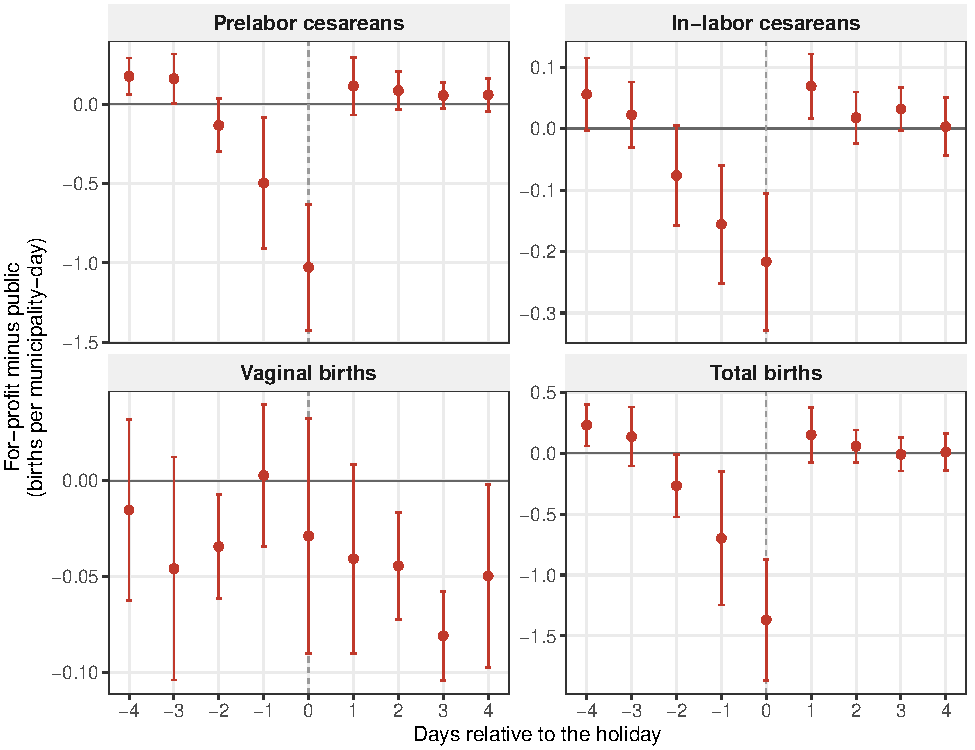
\includegraphics[width=\textwidth]{../analysis/output/graphs/fig_long_weekend_event.pdf}
\caption{\textbf{Delivery counts around bridge holidays}}\label{fig:displacement_event}
\fignotes{Event-study coefficients from Equation~\eqref{eq:event}, 2012--2024,
with 95 percent confidence intervals. Each outcome is the difference in daily
births between for-profit and public establishments within the same municipality,
relative to an ordinary day with the same day of week. The event-time axis runs
from four days before to four days after a bridge holiday. Standard errors are
two-way clustered by municipality and date.}
\end{figure}

\begin{table}[H]
\centering
\caption{\textbf{Alternative long-weekend outcomes and movable holidays}}
\label{tab:displacement_robust}
\small\setlength{\tabcolsep}{5pt}
\begin{tabular}{lcccc}
\toprule
\multicolumn{5}{l}{\emph{Panel A. Event-time sums, share outcomes (percentage points)}} \\
\addlinespace[2pt]
 & \multicolumn{2}{c}{Prelabor cesarean share} & \multicolumn{2}{c}{Cesarean share} \\
\cmidrule(lr){2-3}\cmidrule(lr){4-5}
 & Bridge & Isolated & Bridge & Isolated \\
\midrule
Pre-holiday excess, $\sum_{\ell=-3}^{-1}\theta_\ell$ & -1.933 & -3.097$^{*}$ & -0.057 & 0.084 \\
 & (1.220) & (1.828) & (0.958) & (1.374) \\
\addlinespace[2pt]
Window total, $\sum_{\ell=-3}^{+3}\theta_\ell$ & -9.509$^{***}$ & -11.040$^{***}$ & -0.307 & 1.234 \\
 & (2.169) & (2.956) & (1.821) & (2.379) \\
\addlinespace[2pt]
Observations & 570,180 & 570,180 & 570,180 & 570,180 \\
\midrule
\multicolumn{5}{l}{\emph{Panel B. Prelabor-share taxonomy including movable holidays}} \\
\addlinespace[2pt]
For-profit $\times$ Bridge holiday & \multicolumn{4}{c}{-3.460$^{**}$} \\
 & \multicolumn{4}{c}{(1.744)} \\
\addlinespace[2pt]
For-profit $\times$ Three-day holiday & \multicolumn{4}{c}{-3.564$^{**}$} \\
 & \multicolumn{4}{c}{(1.754)} \\
\addlinespace[2pt]
For-profit $\times$ Isolated holiday & \multicolumn{4}{c}{-4.042$^{*}$} \\
 & \multicolumn{4}{c}{(2.097)} \\
\addlinespace[2pt]
Observations & \multicolumn{4}{c}{4,300,329} \\
\bottomrule
\end{tabular}
\begin{minipage}{\linewidth}\footnotesize
\textit{Notes:} SINASC 2012--2024. Panel A repeats the event study of Table~\ref{tab:long_weekends}, Panel B, with cesarean-share outcomes in place of counts, on the municipality-days on which both sectors record at least one birth; the outcome is the unweighted difference between the for-profit and the public share. Pre-holiday and full-window sums are reported for bridge and isolated holidays. Panel B adds Carnival, Good Friday, and Corpus Christi to the day-of-week holiday taxonomy, a sensitivity analysis outside the fixed-date design: these observances fall on structurally fixed weekdays, which changes the meaning of the holiday-type comparison. Standard errors, two-way clustered by municipality and date, are reported in parentheses.
\newline
\footnotesize Significance levels: *** $p<0.01$, ** $p<0.05$, * $p<0.10$.
\end{minipage}
\end{table}


The negative pre-holiday sums for the prelabor share in Panel A are not evidence of
cesareans being pulled forward, since that prediction requires a positive excess
before the break. The larger negative window sums are consistent with lower
scheduled-delivery intensity across the holiday period, but share-based sums cannot
establish the number of deliveries moved to dates outside the observed window.

\subsection{Organizational capacity}

Larger services can distribute coverage across physicians, use shift-based
arrangements, and maintain operating-room capacity over a wider set of days. They
may therefore have less pronounced weekend declines even if no individual
clinician's preferences change. The regressions interact rest-day indicators with
the establishment's lagged obstetric beds and delivery volume, retaining
establishment-by-year effects. With calendar-date effects only, the weekend
interaction with annual delivery volume is $+1.49$ percentage points per log point
of volume (Table~\ref{tab:org_capacity}). With the stronger municipality-by-date
effects, the volume coefficient falls to $+0.64$ (standard error 0.41) and the bed
coefficient is $+0.58$ (0.38). Neither is individually distinguishable from zero,
but the two are jointly significant (Wald $p = 0.021$). The measures are
correlated but not collinear: their residual interaction correlation is about 0.56
in the stronger specification. Adding municipality-by-date effects substantially
reduces the identifying variation.


\begin{sidewaystable}\centering
   \caption{\label{tab:org_capacity} \textbf{Organizational capacity and prelabor-cesarean timing}}
   \centering
\footnotesize\setlength{\tabcolsep}{3pt}\resizebox{\ifdim\width>\linewidth \linewidth\else\width\fi}{!}{%
   \begin{tabular}{lccccc}
      \toprule
 & (1)            & (2)       & (3)           & (4)           & (5)\\  
\addlinespace[2pt]
 & \multicolumn{3}{c}{Prelabor cesarean share} & Cesarean share & Prelabor cesarean share\\
       & \multicolumn{2}{c}{Prelabor} & Prelabor (terciles) & All cesareans & Prelabor (weak measure) \\ 
      \midrule
      Weekend $\times$ log(1 + obstetric beds)                     & 0.0047         & 0.0058    &               & 0.0059$^{**}$ &   \\   
                                                                   & (0.0035)       & (0.0038)  &               & (0.0026)      &   \\   
\addlinespace[2pt]
      Holiday $\times$ log(1 + obstetric beds)            & 0.0044         & 0.0032    &               & 0.0042$^{*}$  &   \\   
                                                                   & (0.0029)       & (0.0031)  &               & (0.0023)      &   \\   
\addlinespace[2pt]
      Weekend $\times$ log(1 + annual deliveries)                  & 0.0149$^{***}$ & 0.0064    & 0.0105$^{**}$ & 0.0026        & 0.0143$^{***}$\\   
                                                                   & (0.0034)       & (0.0041)  & (0.0043)      & (0.0030)      & (0.0044)\\   
\addlinespace[2pt]
      Holiday $\times$ log(1 + annual deliveries)         & 0.0077$^{**}$  & -0.0041   & -0.0021       & -0.0035       & 0.0002\\   
                                                                   & (0.0031)       & (0.0044)  & (0.0038)      & (0.0035)      & (0.0044)\\   
\addlinespace[2pt]
      Weekend $\times$ middle tercile of beds                      &                &           & -0.0042       &               &   \\   
                                                                   &                &           & (0.0136)      &               &   \\   
\addlinespace[2pt]
      Weekend $\times$ top tercile of beds                         &                &           & 0.0034        &               &   \\   
                                                                   &                &           & (0.0118)      &               &   \\   
\addlinespace[2pt]
      Holiday $\times$ middle tercile of beds             &                &           & 0.0059        &               &   \\   
                                                                   &                &           & (0.0131)      &               &   \\   
\addlinespace[2pt]
      Holiday $\times$ top tercile of beds                &                &           & 0.0068        &               &   \\   
                                                                   &                &           & (0.0099)      &               &   \\   
\addlinespace[2pt]
      Weekend $\times$ log(1 + registered obstetricians)           &                &           &               &               & -0.0038$^{*}$\\   
                                                                   &                &           &               &               & (0.0022)\\   
\addlinespace[2pt]
      Holiday $\times$ log(1 + registered obstetricians)  &                &           &               &               & -0.0020\\   
                                                                   &                &           &               &               & (0.0028)\\   
\addlinespace[2pt]
      \midrule
      Establishment-Year fixed effects & Yes            & Yes       & Yes           & Yes           & Yes\\  
      Date fixed effects & Yes            &           &               &               & \\  
      Municipality-Date fixed effects &                & Yes       & Yes           & Yes           & Yes\\  
      \midrule
      Observations                                                 & 1,192,253      & 1,192,253 & 1,192,253     & 1,192,253     & 1,192,253\\  
      R$^2$                                                        & 0.533          & 0.805     & 0.805         & 0.768         & 0.805\\  
\bottomrule
   \end{tabular}
}
\begin{minipage}{\linewidth}\footnotesize
\textit{Notes:} For-profit SINASC establishment-date cells, 2016--2024, at establishments with at least 50 deliveries in the previous year, weighted by births. The CNES establishment panel begins in 2015, and bed, volume, and staffing measures are lagged one calendar year. All regressions include establishment$\times$year fixed effects. Columns 2--5 add municipality$\times$date fixed effects, which identify the interactions from municipality-days on which more than one for-profit establishment records a birth. The logs of lagged obstetric beds and annual births correlate at 0.48 across establishment-years; net of the fixed effects, the two weekend interactions correlate at 0.64 in column 1 and 0.56 in column 2, so the measures are related but not collinear. In column 2 the weekend interactions are jointly significant (Wald $p=0.021$) although neither is individually. The registered-obstetrician count in column 5 is a weak measure of the obstetric team, because many establishments register no obstetrician under their own CNES code when the physicians are registered elsewhere. These are organizational associations, not effects of exogenously assigned capacity. Standard errors, two-way clustered by establishment and date, are reported in parentheses.
\newline
\footnotesize Significance levels: *** $p<0.01$, ** $p<0.05$, * $p<0.10$.
\end{minipage}
\end{sidewaystable}




Alternative measures in Table~\ref{tab:org_capacity_valid} support an association
with the size of the obstetric service but do not identify a single capacity input.
Replacing headcounts with registered contracted obstetrician hours produces a
weekend interaction of $-0.16$ percentage points (standard error 0.17), while the
volume interaction in that specification is $+1.31$ (0.45). The timing pattern thus
correlates more clearly with service scale than with registered hours in the
obstetrician file. The result may reflect measurement error in those hours rather
than an absence of staffing constraints.

The same table provides one comparison of payment source within the for-profit
ownership class. At the median for-profit establishment, none of the registered
obstetric beds are designated for SUS care. For-profit hospitals with higher SUS
bed shares show flatter weekend and holiday patterns: the interactions for the full
change from zero to 100 percent SUS beds are $+2.58$ and $+2.85$ percentage points.
The hospital's payer exposure is neither random nor fully measured, and the fixed
effects remove only the hospital-year level, not unobserved features whose calendar
gradients covary with SUS participation. This variation shows why ownership and
payer should not be equated; it is not the causal effect of a payer mix.


\begin{sidewaystable}\centering
   \caption{\label{tab:org_capacity_valid} \textbf{Capacity: alternative measures and samples}}
   \centering
\footnotesize\setlength{\tabcolsep}{3pt}\resizebox{\ifdim\width>\linewidth \linewidth\else\width\fi}{!}{%
   \begin{tabular}{lcccccc}
      \toprule
 & (1)                     & (2)                & (3)        & (4)              & (5)              & (6)\\  
\addlinespace[2pt]
 & \multicolumn{6}{c}{Prelabor cesarean share}\\
                                                                        & Beds per 100 deliveries & Larger establishments & Unweighted & No scale control & Contracted hours & Payer exposure \\   
      \midrule
      Weekend $\times$ obstetric beds per 100 deliveries                & 0.0019$^{*}$            &                    &            &                  &                  &   \\   
                                                                        & (0.0010)                &                    &            &                  &                  &   \\   
\addlinespace[2pt]
      Holiday $\times$ obstetric beds per 100 deliveries       & -0.0004                 &                    &            &                  &                  &   \\   
                                                                        & (0.0009)                &                    &            &                  &                  &   \\   
\addlinespace[2pt]
      Weekend $\times$ log(1 + annual deliveries)                       & 0.0130$^{***}$          & 0.0087$^{*}$       & 0.0042     &                  & 0.0131$^{***}$   & 0.0056\\   
                                                                        & (0.0047)                & (0.0050)           & (0.0039)   &                  & (0.0045)         & (0.0045)\\   
\addlinespace[2pt]
      Holiday $\times$ log(1 + annual deliveries)              & -0.0015                 & -0.0039            & -0.0003    &                  & -0.0019          & 0.0037\\   
                                                                        & (0.0040)                & (0.0052)           & (0.0047)   &                  & (0.0044)         & (0.0057)\\   
\addlinespace[2pt]
      Weekend $\times$ log(1 + obstetric beds)                          &                         & 0.0053             & 0.0027     & 0.0080$^{**}$    &                  & 0.0062\\   
                                                                        &                         & (0.0039)           & (0.0032)   & (0.0035)         &                  & (0.0048)\\   
\addlinespace[2pt]
      Holiday $\times$ log(1 + obstetric beds)                 &                         & 0.0033             & 0.0013     & 0.0018           &                  & -0.0103$^{*}$\\   
                                                                        &                         & (0.0032)           & (0.0030)   & (0.0027)         &                  & (0.0053)\\   
\addlinespace[2pt]
      Weekend $\times$ log(1 + contracted obstetrician hours)           &                         &                    &            &                  & -0.0016          &   \\   
                                                                        &                         &                    &            &                  & (0.0017)         &   \\   
\addlinespace[2pt]
      Holiday $\times$ log(1 + contracted obstetrician hours)  &                         &                    &            &                  & 0.0006           &   \\   
                                                                        &                         &                    &            &                  & (0.0020)         &   \\   
\addlinespace[2pt]
      Weekend $\times$ SUS share of obstetric beds                      &                         &                    &            &                  &                  & 0.0258$^{**}$\\   
                                                                        &                         &                    &            &                  &                  & (0.0120)\\   
\addlinespace[2pt]
      Holiday $\times$ SUS share of obstetric beds             &                         &                    &            &                  &                  & 0.0285$^{***}$\\   
                                                                        &                         &                    &            &                  &                  & (0.0106)\\   
\addlinespace[2pt]
      \midrule
      Establishment-Year fixed effects & Yes                     & Yes                & Yes        & Yes              & Yes              & Yes\\  
      Municipality-Date fixed effects & Yes                     & Yes                & Yes        & Yes              & Yes              & Yes\\  
      \midrule
      Observations                                                      & 1,192,253               & 1,017,278          & 1,192,253  & 1,192,253        & 1,192,253        & 1,055,894\\  
      R$^2$                                                             & 0.805                   & 0.803              & 0.804      & 0.805            & 0.805            & 0.824\\  
\bottomrule
   \end{tabular}
}
\begin{minipage}{\linewidth}\footnotesize
\textit{Notes:} Variants of Table~\ref{tab:org_capacity}, column 2. Column 1 substitutes obstetric beds per 100 deliveries in the previous year; column 2 restricts to establishments with at least 200 deliveries in the previous year; column 3 removes the birth weights; column 4 drops annual delivery volume from the controls; and column 5 measures obstetric capacity by the obstetrician hours contracted at the establishment in CNES-PF. Column 6 interacts the rest-day indicators with the share of the establishment's obstetric beds designated for SUS patients. That share is zero at the median for-profit establishment-year, and 21.6 percent of for-profit establishment-years place more than half of their obstetric beds with the SUS. Column 6 excludes establishments with no registered obstetric bed, for which the share is undefined; the SUS share of all beds retains them and yields weekend and holiday interactions of 2.83 (standard error 1.28) and 2.53 (1.06) percentage points. Each capacity measure is lagged one year and its level is absorbed by the establishment$\times$year fixed effects. The establishment link covers 95.4 percent of for-profit births in 2016--2024 (95.3 on weekdays, 95.4 on weekends), and 14.6 percent of the sampled for-profit establishment-years list no obstetrician in CNES-PF. Standard errors, two-way clustered by establishment and date, are reported in parentheses.
\newline
\footnotesize Significance levels: *** $p<0.01$, ** $p<0.05$, * $p<0.10$.
\end{minipage}
\end{sidewaystable}




\subsection{Hospital demand smoothing}\label{app:smoothing}

Scheduling may also benefit a hospital by redistributing delivery volume across
weeks, independently of the individual obstetrician's leisure preferences.
\citet{elejalde2021} identify such an incentive after a shock to hospital demand
in Chile, where cesarean and vaginal deliveries received equal procedure payments.
The Brazilian data permit two observational implications of that mechanism to be
examined, although neither replicates the Chilean identification strategy.

First, hospitals anticipating a busy week should be more likely to bring scheduled
deliveries into the preceding week. Expected demand is constructed for each
establishment and calendar week as the leave-one-out mean of its births in the same
week of the year in other years, after normalizing each year's weekly volume by
that establishment's own average week. Normalization avoids mechanically relating
an excluded year to the other years of a growing or shrinking hospital. Zero-birth
weeks between the establishment's first and last week in each year are retained.
None of the forward-demand coefficients in Table~\ref{tab:demand_smoothing},
Panel A, is distinguishable from zero. The forecast is weak, however: its
out-of-sample slope is only 0.050, and the minimum detectable change is about 0.63
percentage points per log point. A null coefficient therefore places limited
constraints on modest responses to anticipated congestion.

Second, under the demand-smoothing account a stronger tendency to schedule
deliveries should go with less variable week-to-week throughput. Panel B relates
the establishment-year prelabor-cesarean share to the log variance-to-mean ratio of
weekly deliveries, a measure that is zero under a Poisson benchmark and rises as
weekly deliveries become more uneven. The within-establishment estimate is $+0.31$
(standard error 0.16), opposite to the negative sign predicted by leveling. It is
significant at the 10 percent level before adjustment, but not after adjusting
within the family of demand-smoothing tests (Holm $p = 0.173$;
Table~\ref{tab:multiple_testing}). The evidence does not support throughput
leveling in these data; it also does not establish that scheduling causes
deliveries to become more uneven. Both analyses are associational, and the weak
predictive content of expected weekly demand prevents a strong rejection of the
hospital mechanism more generally.

\begin{table}[H]\centering
\caption{\textbf{Anticipated demand and weekly throughput variation}}
\label{tab:demand_smoothing}
\small\setlength{\tabcolsep}{4pt}\resizebox{\ifdim\width>\linewidth \linewidth\else\width\fi}{!}{%
\begin{tabular}{lccccc}
\toprule
\multicolumn{6}{l}{\emph{Panel A. Prelabor timing and expected demand in the following week}} \\
\addlinespace[2pt]
 & \multicolumn{3}{c}{Prelabor cesarean share} & Cesarean share & In-labor share \\
\cmidrule(lr){2-4}\cmidrule(lr){5-5}\cmidrule(lr){6-6}
 & (1) & (2) & (3) & (4) & (5) \\
\midrule
Expected demand, following week & -0.033 & 0.022 & 0.331 & -0.050 & -0.057 \\
 & (0.230) & (0.224) & (0.335) & (0.160) & (0.228) \\
\addlinespace[2pt]
Expected demand, current week & 0.117 & 0.090 & 0.241 & -0.151 & -0.256 \\
 & (0.240) & (0.239) & (0.368) & (0.138) & (0.221) \\
\addlinespace[2pt]
Expected demand, preceding week & 0.267 & 0.022 & 0.130 & 0.010 & -0.175 \\
 & (0.247) & (0.232) & (0.355) & (0.142) & (0.230) \\
\addlinespace[2pt]
\midrule
Establishment fixed effects & Yes & $\times$ year & $\times$ year & $\times$ year & $\times$ year \\
Week-of-year fixed effects & Yes & Yes & -- & Yes & Yes \\
Year fixed effects & Yes & -- & -- & -- & -- \\
Municipality $\times$ week fixed effects & -- & -- & Yes & -- & -- \\
Establishment-weeks & 279,225 & 279,225 & 279,225 & 279,225 & 279,225 \\
Forecast slope, out of sample & \multicolumn{5}{c}{0.050 (0.009)} \\
Minimum detectable $\delta$ (pp) & \multicolumn{5}{c}{0.63} \\
\midrule
\multicolumn{6}{l}{\emph{Panel B. Prelabor scheduling and the dispersion of the weekly delivery flow}} \\
\addlinespace[2pt]
 & \multicolumn{4}{c}{Log variance-to-mean ratio of weekly births} & \\
\cmidrule(lr){2-5}
 & (1) & (2) & (3) & (4) & \\
\midrule
Prelabor cesarean share & 0.059 & 0.311$^{*}$ &  &  & \\
 & (0.133) & (0.164) &  &  & \\
\addlinespace[2pt]
Cesarean share &  &  & 0.256 & 0.659 & \\
 &  &  & (0.255) & (0.595) & \\
\addlinespace[2pt]
Establishment fixed effects & -- & Yes & -- & Yes & \\
Municipality $\times$ year fixed effects & Yes & Yes & Yes & Yes & \\
Establishment-years & 5,319 & 5,319 & 5,319 & 5,319 & \\
\bottomrule
\end{tabular}
}
\begin{minipage}{\linewidth}\footnotesize
\textit{Notes:} For-profit SINASC establishments, 2015--2024, with at least 100 births a year on average and observed in at least five years. Panel A uses establishment-week cells. Expected demand is the establishment's leave-one-year-out mean of births in the same week of the year, each week first normalized by the establishment's mean weekly volume in its own year. Every column controls for the number of holidays in the current and the following week, and coefficients are percentage points of the outcome share per log point of expected demand. The forecast slope is the out-of-sample regression of realized relative demand in the following week on the forecast; the minimum detectable effect assumes 80 percent power and a 5 percent test size. Panel B uses establishment-year cells and the log variance-to-mean ratio of weekly births; its coefficients are log points per unit of the delivery-mode share. Cells are weighted by births. Standard errors are two-way clustered by establishment and week in Panel A and clustered by establishment in Panel B, and are reported in parentheses. These coefficients are associations, not estimates of causal congestion or scheduling effects.
\newline
\footnotesize Significance levels: *** $p<0.01$, ** $p<0.05$, * $p<0.10$.
\end{minipage}
\end{table}


\subsection{Heterogeneity and demand-side alternatives}

An additional scheduling constraint could be the availability of obstetricians in
the municipality. In Table~\ref{tab:heterogeneity} the for-profit weekend dip is
$-6.51$ percentage points in high-density municipalities and $-8.43$ in
low-density municipalities. Physician density is averaged over years at the
municipality level, so its main effect is absorbed by municipality fixed effects;
the coefficient of interest is its interaction with the weekend indicator. The
interaction is consistent with less flexible coverage where obstetricians are
scarcer but is not causal evidence of a staffing mechanism.

Education provides a different split. Among for-profit births, weekday cesarean
rates are much higher for mothers with at least eight years of schooling (85
percent) than for those with fewer years (67 percent). The implied weekend dips
are $-7.22$ and $-11.23$ percentage points, respectively. The regression includes
the education main effect because cells are split by education; otherwise the
difference in levels would contaminate the estimated interaction. The smaller dip
among more-educated mothers could be partly mechanical, because they begin closer
to a cesarean-rate ceiling. It does not rule out demand for scheduled delivery or
differences in access and clinical care.

Physician-owned cooperative insurers offer another observational comparison.
Greater professional control over an insurer might increase discretion over
treatment, but the cooperative indicator is not significantly associated with
cesarean use once municipality and year effects are included. The estimate is
$+0.78$ percentage points with maternal age-band controls (standard error 0.84;
Table~\ref{tab:modality}). Cooperatives differ from other insurers in unobserved
patient and provider characteristics; this null association neither identifies the
effects of provider agency nor rules out patient demand.


\begin{table}[H]
   \caption{\label{tab:heterogeneity} \textbf{Weekend variation by obstetrician density and maternal education}}
   \centering
\small\setlength{\tabcolsep}{5pt}\resizebox{\ifdim\width>\linewidth \linewidth\else\width\fi}{!}{%
   \begin{tabular}{lcc}
      \toprule
 & (1)                     & (2)\\  
\addlinespace[2pt]
 & \multicolumn{2}{c}{Cesarean share}\\
                                                             & By obstetrician density & By mother's education \\   
      \midrule
      Weekend                                                & -0.0651$^{***}$         & -0.1123$^{***}$\\   
                                                             & (0.0056)                & (0.0081)\\   
\addlinespace[2pt]
      Weekend $\times$ low obstetrician density              & -0.0192$^{**}$          &   \\   
                                                             & (0.0076)                &   \\   
\addlinespace[2pt]
      Mother has 8+ years of schooling                       &                         & 0.1090$^{***}$\\   
                                                             &                         & (0.0091)\\   
\addlinespace[2pt]
      Weekend $\times$ mother has 8+ years of schooling      &                         & 0.0401$^{***}$\\   
                                                             &                         & (0.0072)\\   
\addlinespace[2pt]
      Implied dip, high obstetrician density / low education & -0.0651                 & -0.1123\\  
      Implied dip, low obstetrician density / high education & -0.0843                 & -0.0722\\  
      \midrule
      Municipality fixed effects & Yes                     & Yes\\  
      Year fixed effects & Yes                     & Yes\\  
      \midrule
      Observations                                           & 1,312,738               & 1,569,183\\  
\bottomrule
   \end{tabular}
}
\begin{minipage}{\linewidth}\footnotesize
\textit{Notes:} For-profit SINASC municipality-date cells, 2010--2024, weighted by births. Low obstetrician density means below-median registered obstetricians per 1,000 births (CNES register of professionals), using each municipality's mean over the years; its level is absorbed by the municipality fixed effects. The education analysis splits cells at eight years of schooling and includes both the education level and its weekend interaction. The implied-dip rows are linear combinations of the baseline weekend coefficient and the relevant subgroup interaction. Standard errors, two-way clustered by municipality and date, are reported in parentheses.
\newline
\footnotesize Significance levels: *** $p<0.01$, ** $p<0.05$, * $p<0.10$.
\end{minipage}
\end{table}




\begin{table}[H]
   \caption{\label{tab:modality} \textbf{Physician-owned cooperative insurers and cesarean delivery}}
   \centering
\small\setlength{\tabcolsep}{5pt}\resizebox{\ifdim\width>\linewidth \linewidth\else\width\fi}{!}{%
   \begin{tabular}{lcc}
      \toprule
 & (1)       & (2)\\  
\addlinespace[2pt]
 & \multicolumn{2}{c}{Cesarean}\\
      \midrule
      Physician-owned cooperative insurer & 0.0090    & 0.0078\\   
                                          & (0.0085)  & (0.0084)\\   
\addlinespace[2pt]
      Maternal age-band controls          & No        & Yes\\  
      \midrule
      Municipality fixed effects & Yes       & Yes\\  
      Year fixed effects & Yes       & Yes\\  
      \midrule
      Observations                        & 3,408,210 & 3,408,210\\  
\bottomrule
   \end{tabular}
}
\begin{minipage}{\linewidth}\footnotesize
\textit{Notes:} TISS delivery events, 2015--2024. The outcome is cesarean delivery; the explanatory indicator identifies physician-owned cooperative insurers, as opposed to insurer-run plans. Both regressions include municipality and year fixed effects; column 2 adds beneficiary age-band indicators. Standard errors, clustered by municipality, are reported in parentheses.
\end{minipage}
\end{table}




\subsection{Measurement and inference for the fee channel}

Several checks address the measurement of delivery timing and relative physician
fees. The Robson classification cannot independently validate the prelabor
indicator. Groups 1 and 3 require spontaneous labor by definition, and the register
constructs these groups from fields that also enter the before-labor
classification. The zero recorded prelabor share in those groups therefore follows
from the coding rules, not from an external validation of the delivery-timing
variable (Table~\ref{tab:robson_validation}). The remaining information is
narrower. Within Robson group 1, the for-profit weekend cesarean dip is $-6.0$
percentage points. Of this, $-4.7$ points are coded as in-labor cesareans, while
the rest consists of procedures with unavailable timing codes, which may include
prelabor cesareans. The group-1 dip exceeds the group-10 dip by about 1.3 points
($p = 0.006$), although neither group is free of calendar selection.

\begin{table}[H]\centering
\caption{\textbf{Recorded cesarean timing across Robson groups}}
\label{tab:robson_validation}
\small
\small\setlength{\tabcolsep}{4pt}\resizebox{\ifdim\width>\linewidth \linewidth\else\width\fi}{!}{%
\begin{tabular}{lrr}
\toprule
Robson group & Cesareans & Share coded prelabor (\%) \\
\midrule
01 & 1,280,792 & 0.0 \\
02 & 1,883,708 & 84.2 \\
03 &   623,059 & 0.0 \\
04 &   840,859 & 84.9 \\
05 & 3,383,962 & 56.9 \\
06 &   224,461 & 53.7 \\
07 &   306,076 & 52.7 \\
08 &   336,509 & 57.6 \\
09 &    37,321 & 49.9 \\
10 &   891,383 & 55.1 \\
\midrule
\multicolumn{3}{p{0.9\linewidth}}{\footnotesize Group 1 (spontaneous labor) has a 0.0\% prelabor share by construction, since the register assigns every prelabor cesarean of a nulliparous term cephalic singleton to group 2; its for-profit weekend dip of $-6.0$ percentage points therefore has no coded prelabor component: the in-labor component is $-4.7$ percentage points and the remainder is cesareans whose timing code is missing, which the register leaves in group 1 when the prelabor field is blank or ignored, so they may include cesareans performed before labor. The group-1 dip is larger than the group-10 (preterm) dip by 1.3 percentage points ($p=0.006$).} \\
\bottomrule
\end{tabular}
}
\begin{minipage}{\linewidth}\footnotesize
\textit{Notes:} SINASC cesareans in 2014--2024 with a valid before- or during-labor code, by Robson group. Group 1 comprises nulliparous women with a term, singleton, cephalic pregnancy and spontaneous labor; group 2 the corresponding women with induced labor or prelabor cesarean. Because the register uses labor onset and cesarean timing to assign Robson groups, the zero prelabor shares in groups 1 and 3 hold by construction. Within group 1, incomplete timing coding prevents attributing the full weekend dip to prelabor or in-labor procedures. The group-1 versus group-10 comparison is descriptive, and preterm deliveries can also be planned.
\end{minipage}
\end{table}


The fee-gap coefficients also require care in interpretation. The municipal and
state fixed-effect estimates differ in sign, and the latter rest on only 27 state
clusters in the levels models. Table~\ref{tab:feegap_ci} tests a defined
economic-equivalence region and compares the coefficient intervals with two
external estimates of the response to physician fees. None of the intervals lies
wholly within the equivalence region of $\pm 0.02$, so the data do not establish an
economically negligible response. The municipality fixed-effect intervals exclude
both the \citet{grant2009} and the \citet{gruber1999physician} reference
magnitudes; the state fixed-effect intervals exclude neither. The observational
regressions therefore do not deliver a stable estimate of how Brazilian physicians
would respond to a fee reform.

\begin{sidewaystable}\centering
\caption{\textbf{The fee-gap coefficient, an equivalence region, and the literature's price responses}}
\label{tab:feegap_ci}
\small
\small\setlength{\tabcolsep}{4pt}\resizebox{\ifdim\width>\linewidth \linewidth\else\width\fi}{!}{%
\begin{tabular}{lcccccc}
\toprule
Specification & Coefficient & 95\% CI & Clusters & In $[-0.02,0.02]$? & Excludes Grant? & Excludes GKM?
\\
\midrule
State fixed effects & +0.0488 & [+0.0006, +0.0970] &  27 & not within & not excluded & not excluded \\
Municipality fixed effects & -0.0141 & [-0.0301, +0.0020] & 721 & not within & excluded & excluded \\
State fixed effects + controls & +0.0190 & [-0.0296, +0.0675] &  27 & not within & not excluded & not excluded \\
Municipality fixed effects + controls & -0.0125 & [-0.0284, +0.0035] & 716 & not within & excluded & excluded \\
\bottomrule
\end{tabular}
}
\begin{minipage}{\linewidth}\footnotesize
\textit{Notes:} Coefficient on the log economic fee gap from Table~\ref{tab:fees}. The equivalence region $[-0.02, 0.02]$ corresponds to a 2 percentage-point change in the cesarean share per log point of the fee gap. The final two columns ask whether the interval excludes the price response the literature has estimated. \citet{gruber1999physician} report about four percentage points of cesarean rate per US\$1{,}000 of the cesarean-vaginal fee differential; re-estimating that response on corrected data, \citet{grant2009} obtains about one point, which he describes as a quarter of the original. At our delivery-weighted mean cesarean fee of R\$1,963 the two are 0.75 and 3.01 percentage points per log point of the fee gap. That fee is the mean over the municipality-years of Table~\ref{tab:fees}, weighted by deliveries; the mean over delivery events that Table~\ref{tab:fee_per_hour} and the text report, R\$1,939, is 1 percent lower and would put them at 0.74 and 2.97. The conversion uses US consumer prices between 1990 and 2020 and the World Bank purchasing-power factor for Brazil, and is deliberately rough. The calibration uses nominal mean fees over 2015--2024. Using IPCA-deflated fees expressed in 2020 reais yields reference magnitudes of 0.74 and 2.94 percentage points per log point for \citet{grant2009} and \citet{gruber1999physician}, respectively, compared with 0.75 and 3.01 in the baseline. No confidence-interval comparison changes. Two things follow, and the paper states both. No interval fits inside the equivalence region, so these data do not establish that the price response is negligible. And the two fixed-effect schemes disagree about both magnitudes: the within-municipality intervals exclude them, the state-level intervals, estimated on 27 clusters, are too wide to. The sign itself is unstable across the two schemes. The economic argument of Section~\ref{sec:notprice} does not rest on this table: the 0.20 to 0.49 log point negative fee gap of the largest states would move the cesarean rate by at most about 0.37 percentage points at Grant's magnitude and 1.5 at the original, against a for-profit--public gap of 36 points.
\end{minipage}
\end{sidewaystable}

% a sidewaystable floats to the next page while [H] tables print in place;
% the barrier keeps the numbering and the page order the same
\FloatBarrier

The fee sign reversal is not caused by the separately billed labor-assistance
component alone. Re-estimating the same municipality-year regressions with the base
vaginal delivery fee produces a positive state fixed-effect coefficient ($+0.0366$)
and a negative municipality fixed-effect coefficient ($-0.0176$), the same pattern
as the economic-fee specification (Table~\ref{tab:fee_base_econ}). The sensitivity
addresses the construction of the fee measure; it does not resolve the endogeneity
of fees or unobserved differences in the local obstetric market.


\begin{table}[H]
   \caption{\label{tab:fee_base_econ} \textbf{Fee-gap estimates using base and economic vaginal fees}}
   \centering
\small\setlength{\tabcolsep}{4pt}\resizebox{\ifdim\width>\linewidth \linewidth\else\width\fi}{!}{%
   \begin{tabular}{lcccc}
      \toprule
 & (1)          & (2)            & (3)           & (4)\\  
\addlinespace[2pt]
 & \multicolumn{4}{c}{Private-insurance cesarean rate}\\
       & \multicolumn{2}{c}{Base vaginal fee} & \multicolumn{2}{c}{Economic vaginal fee} \\ 
      \midrule
      Log fee gap (base vaginal fee)     & 0.0366$^{*}$ & -0.0176$^{**}$ &               &   \\   
                                         & (0.0179)     & (0.0081)       &               &   \\   
\addlinespace[2pt]
      Log fee gap (economic vaginal fee) &              &                & 0.0488$^{**}$ & -0.0141$^{*}$\\   
                                         &              &                & (0.0235)      & (0.0082)\\   
\addlinespace[2pt]
      \midrule
      State fixed effects & Yes          &                & Yes           & \\  
      Year fixed effects & Yes          & Yes            & Yes           & Yes\\  
      Municipality fixed effects &              & Yes            &               & Yes\\  
      \midrule
      Observations                       & 5,198        & 5,198          & 5,198         & 5,198\\  
      R$^2$                              & 0.332        & 0.855          & 0.354         & 0.855\\  
\bottomrule
   \end{tabular}
}
\begin{minipage}{\linewidth}\footnotesize
\textit{Notes:} Private-insurance municipality-years with at least 20 deliveries, weighted by deliveries. Columns 3--4 reproduce Table~\ref{tab:fees}, columns 1--2, with the economic vaginal fee (the procedure fee plus any separately billed labor assistance). Columns 1--2 use only the base vaginal procedure fee and keep the same municipality-years, outcome, and weights. Standard errors, clustered by the fixed-effect geography, are reported in parentheses.
\newline
\footnotesize Significance levels: *** $p<0.01$, ** $p<0.05$, * $p<0.10$.
\end{minipage}
\end{table}




The difference between payment per delivery and compensation per hour is
illustrated in Table~\ref{tab:fee_per_hour}. Among vaginal deliveries with a
positive base delivery fee, 40.5 percent also bill hourly labor assistance. Their
mean economic physician fee is R\$3,355, compared with R\$1,778 for those billing
none. The average over that same population is R\$2,417, so the billing share and
the conditional fee means reconcile. The mean cesarean fee over events with a
positive delivery fee is R\$1,939. These figures are billed physician fees, not the
full opportunity cost or realized net earnings. The expected vaginal fee at the
time the mode is chosen is not necessarily the fee of the delivery subsequently
observed.

Assuming a cesarean occupies one hour of physician time, the mean economic vaginal
fee yields a break-even vaginal attendance time of about 1.25 hours; the thresholds
are 1.73 hours among vaginal deliveries billing labor assistance and 0.92 hours
among those billing none. For a two-hour cesarean, the aggregate threshold is about
2.49 hours. Because billed hours do not measure total physician time, these are
illustrative comparisons, not estimated time costs.

\begin{table}[H]
\centering
\caption{\textbf{Physician fees per delivery and per hour of physician time}}
\label{tab:fee_per_hour}
\small\setlength{\tabcolsep}{5pt}
\resizebox{\ifdim\width>\linewidth \linewidth\else\width\fi}{!}{%
\begin{tabular}{lcccccc}
\toprule
 & Brazil & SP & MG & RJ & PR & SC \\
\midrule
\multicolumn{7}{l}{\emph{Panel A. Fees per delivery (R\$)}} \\
\addlinespace[2pt]
Cesarean fee & 1,939 & 1,894 & 1,928 & 2,244 & 1,690 & 1,878 \\
Vaginal delivery fee alone & 1,893 & 2,169 & 1,933 & 2,545 & 1,445 & 1,422 \\
Economic vaginal fee, all vaginal deliveries & 2,417 & 2,399 & 3,133 & 2,845 & 2,060 & 2,319 \\
\quad deliveries billing labor assistance & 3,355 & 3,842 & 3,788 & 4,162 & 2,518 & 2,942 \\
\quad deliveries billing none & 1,778 & 2,036 & 1,507 & 2,374 & 1,206 & 1,188 \\
\midrule
\multicolumn{7}{l}{\emph{Panel B. Labor assistance}} \\
\addlinespace[2pt]
Vaginal deliveries billing labor assistance (\%) & 40.5 & 20.1 & 71.3 & 26.4 & 65.1 & 64.5 \\
Billed hours, when billed & 2.9 & 2.7 & 3.3 & 2.4 & 3.0 & 3.2 \\
Fee per billed labor hour (R\$) & 420 & 404 & 496 & 476 & 315 & 429 \\
\midrule
\multicolumn{7}{l}{\emph{Panel C. Break-even physician time of a vaginal delivery (hours)}} \\
\addlinespace[2pt]
If a cesarean takes one hour & 1.25 & 1.27 & 1.62 & 1.27 & 1.22 & 1.23 \\
\quad deliveries billing labor assistance & 1.73 & 2.03 & 1.96 & 1.85 & 1.49 & 1.57 \\
\quad deliveries billing none & 0.92 & 1.07 & 0.78 & 1.06 & 0.71 & 0.63 \\
If a cesarean takes two hours & 2.49 & 2.53 & 3.25 & 2.54 & 2.44 & 2.47 \\
\bottomrule
\end{tabular}}
\begin{minipage}{\linewidth}\footnotesize
\textit{Notes:} TISS private-insurance deliveries, 2015--2024; the five largest
states by deliveries, as in Section~\ref{sec:notprice}. Fees are means over the
deliveries that bill them: the cesarean fee over cesareans with a positive
delivery fee, the vaginal fees over vaginal deliveries with a positive delivery
fee (94.2 percent of vaginal deliveries nationally). The economic
vaginal fee is, for each such delivery, the delivery fee plus
the hourly labor-assistance fee billed with it, counted as zero where none is
billed, averaged over all of them. It is the expected pay of a vaginal delivery
when the mode of delivery is chosen, not the pay of a typical one: the two rows
below it split it by whether labor assistance is billed, and a vaginal delivery
that bills none pays less than a cesarean in Brazil as a whole. The fee per
billed labor hour is the mean, over the deliveries that bill labor assistance, of
that fee divided by its billed hours. Panel C reports the physician time of a
vaginal delivery at which the economic vaginal fee per hour equals the cesarean
fee per hour: the economic vaginal fee divided by the cesarean fee, times the
hours of a cesarean; the two indented rows apply the same ratio to the two
kinds of vaginal delivery, so the first row holds for the expected fee only. A
vaginal delivery that occupies the physician for longer than its threshold
pays less per hour than a cesarean. Physician time is not observed; billed hours
are a floor on it, since the vaginal deliveries that bill no labor hours still
take time (60 percent of them nationally, between 29 and 80 percent in
the five states), so the comparison is tilted in favor of the vaginal delivery.
Fee amounts are nominal means over 2015--2024. Deflating annual fees to 2020 reais using the IPCA leaves every comparison drawn in the text unchanged and reduces the one-hour cesarean break-even threshold from 1.25 to 1.22 hours.
Reais convert to US dollars at about R\$4.37 per dollar, the mean official exchange rate of 2015--2024.
\end{minipage}
\end{table}


Because the state-level fee-shock analysis has few geographic clusters,
conventional asymptotic inference warrants a separate check. The first-difference
coefficient is $-0.0087$; its conventional cluster-robust $p$-value is 0.351, and a
Webb-weight wild-cluster bootstrap with 9,999 draws \citep{cameron2008,webb2023}
gives $p = 0.323$ (Table~\ref{tab:fewcluster}). Neither calculation rejects zero,
and neither establishes that the causal fee effect is absent.

\begin{table}[H]\centering
\caption{\textbf{Few-cluster inference for the fee-shock specification}}
\label{tab:fewcluster}
\small
\small\setlength{\tabcolsep}{4pt}\resizebox{\ifdim\width>\linewidth \linewidth\else\width\fi}{!}{%
\begin{tabular}{lc}
\toprule
Quantity & Value \\
\midrule
Fee-shock coefficient ($\Delta$ cesarean on $\Delta$ fee gap) & -0.0087 \\
Number of state clusters & 22 \\
Cluster-robust analytic $p$-value & 0.351 \\
Wild-cluster (Webb) bootstrap $p$-value & 0.323 \\
\bottomrule
\end{tabular}
}
\begin{minipage}{\linewidth}\footnotesize
\textit{Notes:} State-year first differences, weighted by TISS deliveries. The bootstrap uses 9,999 Webb-weight draws with states as clusters. The number of state clusters differs from the state-level levels models of Table~\ref{tab:feegap_ci} because the first-difference design has a different sample. The municipality fixed-effect specifications of Table~\ref{tab:fees} have hundreds of clusters and are not the focus of this check.
\end{minipage}
\end{table}

\begin{table}[H]\centering
\caption{\textbf{Sample construction for the SINASC analyses}}
\label{tab:sampleflow}
\small
\small\setlength{\tabcolsep}{4pt}\resizebox{\ifdim\width>\linewidth \linewidth\else\width\fi}{!}{%
\begin{tabular}{lr}
\toprule
Step & Records \\
\midrule
Raw SINASC birth records & 42,006,849 \\
Restrict to 2010--2024 & 42,006,849 \\
For-profit or public establishment & 26,505,312 \\
\quad of which: 2014--2024 with a valid Robson group & 18,822,989 \\
\quad of which: cesareans, 2010--2024 & 14,644,214 \\
\quad\quad of which: 2012--2024 & 12,823,213 \\
\quad\quad\quad of which: valid before/during-labor code & 11,709,002 \\
\bottomrule
\end{tabular}
}
\begin{minipage}{\linewidth}\footnotesize
\textit{Notes:} The Robson-classified row and the cesarean row are separate subsets of all for-profit and public births, not nested subsets of each other; the timing-code rows are nested within cesareans. Delivery-timing analyses use 2012 onward and Robson analyses 2014 onward. Sample sizes differ across exhibits with the availability of each outcome.
\end{minipage}
\end{table}

\begin{table}[H]\centering
\caption{\textbf{Missing timing codes by sector and day type}}
\label{tab:timing_missing}
\small
\small\setlength{\tabcolsep}{4pt}\resizebox{\ifdim\width>\linewidth \linewidth\else\width\fi}{!}{%
\begin{tabular}{lcc}
\toprule
Sector & Weekday (\%) & Weekend (\%) \\
\midrule
For-profit & 6.81 & 6.71 \\
Public & 10.34 & 10.31 \\
\bottomrule
\end{tabular}
}
\begin{minipage}{\linewidth}\footnotesize
\textit{Notes:} Share of SINASC cesareans with a missing before- or during-labor code, 2012--2024. At the sector level the shares differ little between weekdays and weekends. This does not establish valid measurement within every Robson group: among for-profit cesareans assigned to group 1, the code is missing more often on weekdays (11.2 percent) than on weekends (9.8 percent) in 2014--2024, so part of that group's weekend dip may involve uncoded prelabor cesareans (Table~\ref{tab:robson_validation}).
\end{minipage}
\end{table}


\subsection{Multiple hypothesis testing}\label{app:multiple}

The paper reports several related hypotheses in the calendar regressions and
supplementary analyses. Rather than reading each unadjusted $p$-value as a separate
confirmatory test, Table~\ref{tab:multiple_testing} groups the reported tests into
six substantive families. Within each family, the step-down adjustment of
\citet{holm1979} controls the familywise error rate, and the \citet{benjamini1995}
$q$-value controls the expected false discovery rate. The families follow the
empirical questions, not whether individual results are significant. These
adjustments do not repair bias or turn observational coefficients into causal
effects; they address the risk of chance significance from testing several related
coefficients.

The headline for-profit calendar interactions in family A of
Table~\ref{tab:multiple_testing} and the for-profit--public
outcome differences in family C remain significant after correction. In family B
the obstetrician-density and education interactions remain significant and the
cooperative-insurer contrast does not. In family D the four ordinary fixed-date
long-weekend hypotheses have unadjusted $p$-values between 0.05 and 0.07 and Holm
values of 0.20, so none is significant on its own after adjustment. Family E
includes both bed and volume interactions from the same specification, none of
which is individually significant; estimates for either capacity measure entered
alone are a different exercise (Table~\ref{tab:org_capacity_valid}). In family F,
the weakly positive throughput-dispersion association does not survive adjustment
(Holm $p = 0.173$), and neither forward-demand coefficient is significant. The
results support a robust weekly calendar pattern and do not confirm the specific
holiday-leisure and weekly-throughput predictions.

\begin{table}[H]
   \caption{\label{tab:multiple_testing} \textbf{Adjusted inference within hypothesis families}}
   \centering
\small\setlength{\tabcolsep}{5pt}\resizebox{\ifdim\width>\linewidth \linewidth\else\width\fi}{!}{%
   \begin{tabular}{lcccc}
      \toprule
      Hypothesis & Estimate & Unadjusted $p$ & Holm $p$ & BH $q$ \\
      \midrule
      \emph{A. For-profit calendar gradient} & & & & \\
      \quad For-profit $\times$ Weekend & -0.0179 & 0.004 & 0.004 & 0.004 \\
      \quad For-profit $\times$ Holiday & -0.0255 & $<$0.001 & $<$0.001 & $<$0.001 \\
      \quad For-profit $\times$ Eve of rest day & -0.0106 & 0.002 & 0.003 & 0.002 \\
      \addlinespace[3pt]
      \emph{B. Heterogeneity in the weekend dip} & & & & \\
      \quad Weekend $\times$ Low obstetrician density & -0.0192 & 0.011 & 0.023 & 0.017 \\
      \quad Weekend $\times$ Mother has 8+ years of schooling & 0.0401 & $<$0.001 & $<$0.001 & $<$0.001 \\
      \quad Physician-owned cooperative insurer & 0.0078 & 0.355 & 0.355 & 0.355 \\
      \addlinespace[3pt]
      \emph{C. For-profit--public outcome differences} & & & & \\
      \quad Early-term birth (37--38 weeks) & 0.1218 & $<$0.001 & $<$0.001 & $<$0.001 \\
      \quad Low birthweight ($<$2500g) & -0.0347 & $<$0.001 & $<$0.001 & $<$0.001 \\
      \quad Five-minute Apgar $<$ 7 & -0.0063 & $<$0.001 & $<$0.001 & $<$0.001 \\
      \addlinespace[3pt]
      \emph{D. Long weekends} & & & & \\
      \quad For-profit $\times$ Bridge holiday & -0.0339 & 0.060 & 0.202 & 0.070 \\
      \quad For-profit $\times$ Three-day holiday & -0.0362 & 0.051 & 0.202 & 0.070 \\
      \quad For-profit $\times$ Isolated holiday & -0.0404 & 0.054 & 0.202 & 0.070 \\
      \quad Pre-holiday excess, prelabor cesareans & -0.4684 & 0.070 & 0.202 & 0.070 \\
      \addlinespace[3pt]
      \emph{E. Organizational capacity} & & & & \\
      \quad Weekend $\times$ log(1 + obstetric beds) & 0.0058 & 0.131 & 0.484 & 0.262 \\
      \quad Holiday $\times$ log(1 + obstetric beds) & 0.0032 & 0.296 & 0.592 & 0.350 \\
      \quad Weekend $\times$ log(1 + annual deliveries) & 0.0064 & 0.121 & 0.484 & 0.262 \\
      \quad Holiday $\times$ log(1 + annual deliveries) & -0.0041 & 0.350 & 0.592 & 0.350 \\
      \addlinespace[3pt]
      \emph{F. Demand smoothing} & & & & \\
      \quad Expected demand next week $\times$ prelabor cesarean share & 0.0002 & 0.922 & 1.000 & 0.922 \\
      \quad Expected demand next week $\times$ cesarean share & -0.0005 & 0.757 & 1.000 & 0.922 \\
      \quad Prelabor cesarean share $\times$ weekly flow dispersion & 0.3114 & 0.058 & 0.173 & 0.173 \\
      \addlinespace[3pt]
\bottomrule
   \end{tabular}
}
\begin{minipage}{\linewidth}\footnotesize
\textit{Notes:} Family A corresponds to Table~\ref{tab:main_gradient}; B to Tables~\ref{tab:heterogeneity}--\ref{tab:modality}; C to Table~\ref{tab:health}; D to Table~\ref{tab:long_weekends}; E to Table~\ref{tab:org_capacity}; and F to Table~\ref{tab:demand_smoothing}. Holm $p$-values \citep{holm1979} adjust within each family and control its familywise error rate; Benjamini--Hochberg $q$-values \citep{benjamini1995} target the false discovery rate. Estimates and unadjusted $p$-values reproduce the source exhibits.
\end{minipage}
\end{table}



% =============================================================================
\section{The policy record}\label{app:policy}
% =============================================================================

Brazilian reforms have tried to change cesarean decisions through reimbursement
rules, information, and quality improvement. Two episodes are informative about
institutional implementation, but neither identifies the causal effect of a policy.
A December 2015 judicial order called for private plans to pay at least three
times as much for vaginal delivery as for cesarean delivery. The regulator
appealed, and the directive did not produce an implemented change in the relative
fee schedule (Section~\ref{sec:notprice}). The order therefore cannot be used as an
exogenous price shock or as evidence that a change in relative fees failed to
affect delivery decisions.

The second episode is Parto Adequado, a quality-improvement initiative that
hospitals joined between 2017 and 2021. The public participant list does not
provide a reliable hospital-specific start date. Figure~\ref{fig:pa_hospital}
imposes a common 2017 onset and compares the cesarean rates of participating and
nonparticipating for-profit hospitals over the long pre-period the birth records
afford, using the interaction-weighted event study of \citet{sun2021}. With a
single imposed adoption date there is only one treated cohort, so the estimator is
equivalent to a two-way fixed-effects event study against never-participating
hospitals; it cannot correct for the unknown staggered entry dates.

The participating hospitals exhibit a downward differential trend well before the
assumed onset, without a distinct break at 2017, so post-onset declines cannot be
attributed to the program from this comparison. The decline is consistent with
improvement but does not isolate a program effect, which cautions against causal
readings of short before-and-after comparisons, including the improvement
associated with participation in \citet{borem2020}.
Figure~\ref{fig:rn368} provides the national monthly series and marks the 2015
disclosure regulation as institutional background, not as an event-study
treatment.

\begin{figure}[H]\centering
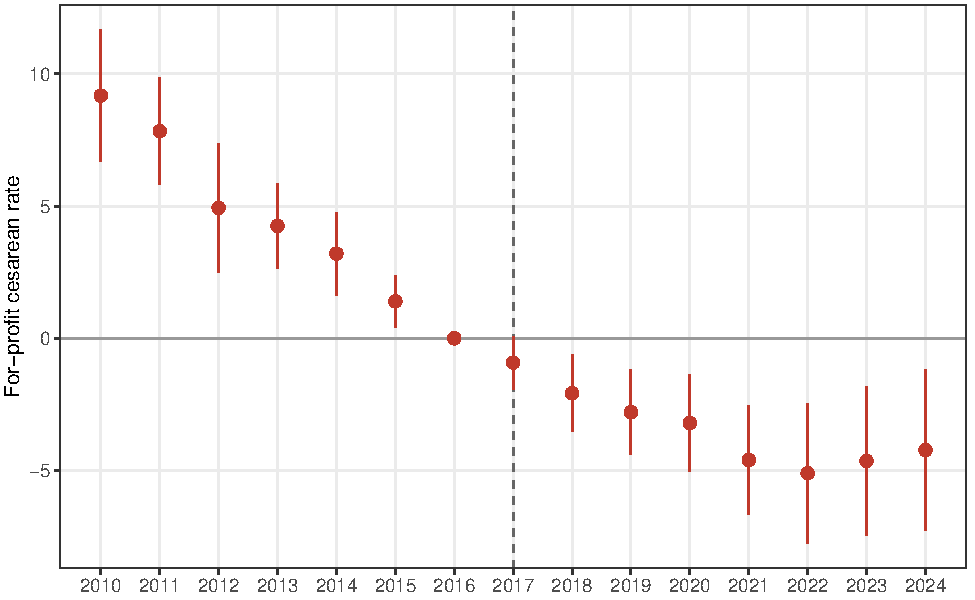
\includegraphics[width=\textwidth]{../analysis/output/graphs/fig_ref_c11_pa_hospital_es.pdf}
\caption{\textbf{Cesarean-rate trends in Parto Adequado hospitals}}\label{fig:pa_hospital}
\fignotes{Hospital-level comparison between participating and nonparticipating
for-profit establishments, with a common assumed onset in 2017 and the preceding
year as reference. The interaction-weighted coefficients of \citet{sun2021} are
numerically equivalent to a two-way fixed-effects event study with one cohort and
never-participating controls. Participating hospitals were already on a
differential downward trend before 2017. Without hospital-specific entry dates, the
figure cannot identify the program's effect or represent staggered implementation.}
\end{figure}

\begin{figure}[H]\centering
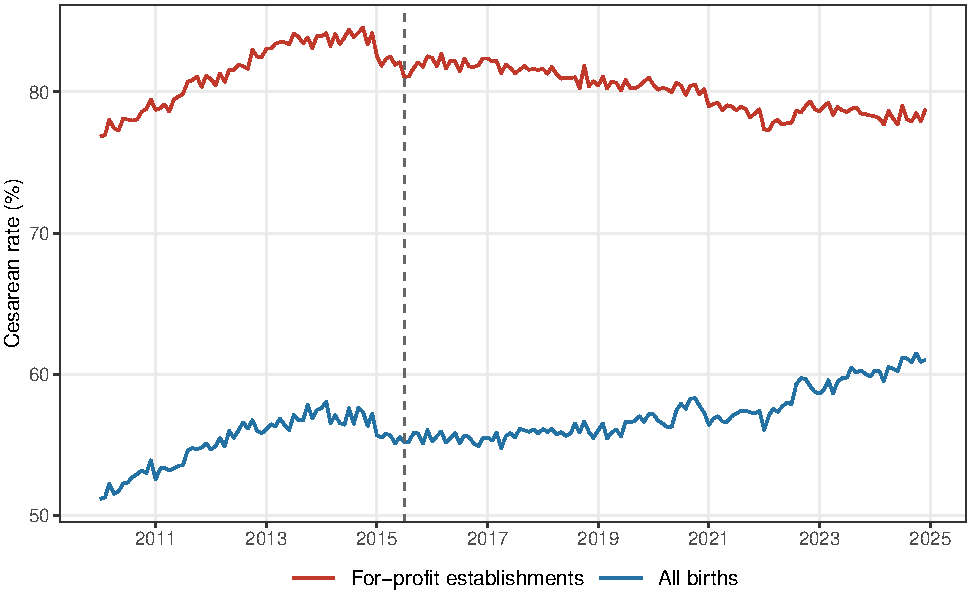
\includegraphics[width=\textwidth]{../analysis/output/graphs/fig05_rn368_timeline.pdf}
\caption{\textbf{National cesarean rates and the regulatory timeline}}\label{fig:rn368}
\fignotes{Monthly SINASC cesarean shares among all births and among births in
for-profit establishments. The vertical line marks ANS Resolution RN 368/2015. The
series is descriptive and is not an interrupted time-series estimate of the
regulation's effect.}
\end{figure}
